\chapter{Classifying Superluminous Supernova using Machine Learning}
\label{Chapter5}
\lhead{Chapter 5. \emph{ML Classification}}

\begin{figure}[H]
  
\includegraphics{Figures/xkcd/chapter5.png}
  \caption*{xkcd.com/1838}
\end{figure}

SN classifications, focusing particularly on the selection of SLSNe, formed the underlying theme of this thesis. In \cref{Chapter4}, I established a definition of SLSNe in terms of the parameter space of the spin-down of a Magnetar model, later used to photometrically classify one SLSN in the SNLS archival data. In this chapter, I begin by describing the application of this previously successful technique to the DES dataset, performed in real-time during the seasons two and three of DES. This included both the manual scanning of SNe and combining it with the Magnetar model fitting. While successful in identifying several candidates, and later spectroscopically confirmed, SLSNe, a number of misclassifications highlighted a need for a more robust approach.

In recent years the field of astronomy entered a new data analysis renaissance, utilising Big Data tools and Machine Learning techniques to extract more from archival data and prepare for the arrival of new surveys such as Gaia, ZTF, LSST and SKA that are expected to produce staggering amounts of data, exceeding everything that we were familiar with in the past decades. Beside creating difficulties in their analysis, the streaming, handling and storing of the data is also a serious issue requiring state-of-the-art facilities and tools. Following in the footsteps of this revolution, I endeavoured to apply some of the latest ML techniques that are proven in other fields as well as in real-world applications, to the problem of SN classification.

To date, there has been a number of studies aiming to classify SNe with the help of ML. In this thesis, I am focusing only on the studies classifying the light curves of SNe and not point source classification pipelines such the once used recently in DES \citep{Goldstein2015} and Suburu \citep{Morii2014}. Amongst a number of similar works \citep{Karpenka2012,Moller2016,Charnock2016} the most thorough and in-depth study is presented in \citet{Lochner2016}. In their work, a number of models are used to extract a broad range of light curve features. They also provide a comparison of a number of Supervised ML algorithms and discuss their merits in terms of SN classification. While thorough in their analysis, their approach is not ready for deployment in a real survey. The training sample used in their analysis is the SPCC dataset containing a sanitised sample of SNe only. In a survey such as DES, we are faced with sample heavily contaminated by other classes of transients.

The use of the SPCC dataset by \citet{Lochner2016} containing only 2000 SNe, weighted to match their expected spectroscopic classification rates, is one of their greatest drawbacks. In this thesis, I aim to provide the first SN classification approach utilising a large (tens of thousands of objects for each subclass), artificially generated sample of objects. With the size of the training sample, I tackle the common issue with overfitting for the less common subclasses of SNe. Furthermore, by placing the SNe uniformly throughout the DES observing season and at a wide range of redshifts, I produce realistic survey imperfections, including objects which suffer from season edge effects and low S/N.

One of the greatest differences between all previous studies and this thesis is the family of ML algorithms used. \citet{Lochner2016} used the SALT2 model and wavelet decomposition, in a process commonly referred to in ML as Feature Extraction or Feature Engineering, to extract a set of parameters that describe the light curve. These are then fed into the ML algorithms to produce their classifications. In this thesis, I use Convolutional Neural Networks (CNN), a powerful technique which dominates the world of commercial ML solutions. CNNs, described in detail in \sref{sec:CNN}, use the data directly as they build their own bespoke feature sets as part of the learning process. The use of such a complex ML tool is only possible thanks to the extent of the training sample along with the data augmentation described in \sref{sec:DataAugmentation}.

In this chapter, I describe the process of creating an artificial training sample of SNe for a majority of their dominant subclasses, based on the tools developed in \cref{Chapter3}, as well as AGNs and noise spikes which form the majority of transients detected by DES. Following from this, I describe the steps taken to apply the survey noise model to the otherwise smooth, simulated data before interpolating and augmenting it with the help of GPR, described in \sref{sec:GP}. Finally, I discuss the use of the CNN framework to provide a photometric classification for all transients detected by DES in the first four years of its operations.

\section{Traditional Approach to Searching for SLSN in DES}
Before applying the ML framework to the problem of selecting SLSN, I have used the magnetar model approach originally developed in \cref{Chapter4} for the use of the SNLS data. This gave us some encouraging results, providing the classification for several SLSNe in the DES data, however, the subsequent discoveries of a number of objects that do not fit the known models, including cases such as DES15S2nr, demonstrated the need for a different approach.

\subsection{Magnetar Model Fitting}
A major difference between the approaches used to identify SLSN in DES and that of SNLS is the completeness and the stage at which the data enters the analysis pipeline. In \cref{Chapter4} I applied the techniques retrospectively to archival data. This, outside limited cases suffering from season edge effects, gave me a sample of near complete light curves that could be modelled with a much higher confidence rate. In DES, I attempted to model the light curves during their early rise phases. This was a constraint dictated not only by our desire to classify the objects at the earliest possible phase (as early time spectra of SLSNe are still not sufficiently abundant) but also due to the computational resources required to fit all the light curves in real-time. Despite a number of optimisations applied to our fitting routine (\sref{sec:SLAP}), I was limited to fitting data detected within last three to four observing epochs. As it is not possible to constrain such a complex model with less than three epoch of multi-band data, I have delayed the analysis of each object until the first epoch where at least three observations, in a minimum of three photometric bands, are available. If the object remained active (i.e detected in the latest of the three epochs), I attempted to fit the magnetar model to it and compare the result against the definition of SLSNe. I have subsequently repeated this step, up to the maximum of four times, when new data became available. At that stage, if the object did not match our definition in any of the epoch of fitting it was discarded.

\subsubsection{Problems}
A number of problems revolving around this approach were uncovered during the DES runs that resulted in a number misclassifications of SLSNe, both as true-negatives and false-positives.

\paragraph{`Bumpy' SLSNe}
One of the drawbacks of the rules put in place in order to optimise the fitting process and reduce the number of false detections being passed through the classification pipeline is the rejection of some objects, most predominantly DES15C3hav, which show a slowly evolving pre-peak bump close to the detection limit of the survey (Angus et al; in prep). In the case of DES15C3hav, the early activity was only detected in two consecutive epochs before the S/N of the light curve dropped considerably for a number of weeks prior to the rebrightening at the onset of the main SLSN event.

Similarly, while no such cases have been identified, it is also likely that a pre-peak bump, similar to that found in DES14X3taz \citep{Smith2016}, would have been excluded by these cuts as its initial seven epochs do not give a good fit to the magnetar model and do not fit the definition of SLSNe.

\paragraph{Faint SLSNe}
One of the most interesting discoveries made about the population of SLSNe is the abundance of objects which, while spectroscopically consistent with the published population of SLSNe, are found at absolute luminosities lower than previously expected, as faint as M$\sim$-19. From \citet{Inserra2018a} and \citet{Nicholl2014, Nicholl2017}, we know that the evolution of SLSNe, both in terms of the rise and decline time, is strongly linked with their luminosity resulting in the different morphology of the fainter events. As no such objects were known at the time, they were not present in the sample used in \cref{Chapter4}, resulting in a strong bias of the magnetar model definition against such objects. This resulted in a number of fainter SLSNe (for example DES14C1rhg) to be overlooked.

\paragraph{Lack of late-time data}
Perhaps one of the most important issues with this approach is the assertion that it is possible to model a SLSNe using its rise-time data alone. It was shown in \citet{Inserra2013} and \citet{Inserra2018a} that SLSNe is most strongly characterised by their late-time light curve. This became apparent amongst the DES sample of SLSNe upon the discovery of DES15E2mlf, the most distant spectroscopically confirmed SLSN at the point of its classification \citep{Pan2017}. The visual inspections, the search described in this section as well as the standard DES SN template fitting, have strongly suggested that the object is a SN\,Ia at z$\sim$0.3. With a rapid rise and a relatively bright host galaxy, a SLSN classification appeared counter-intuitive; however, our subsequent analysis in \citet{Pan2017} showed that at high redshift we are sampling the UV regions of the SED where the evolution of SLSNe are a lot more rapid due to rapid cooling of the photosphere in the early phases. Similarly, the host galaxy was found to be consistent with a heavily star-forming galaxy, often associated with SLSNe, explaining the excess UV luminosity.

\section{Training sample} \label{sec:TrainingSample}
In any ML project, the data sample used to train the classification model is its most important element. Regardless of the algorithm used, without correct and representative samples, the model will not be able to accurately label new data and often may result in overfitting. An ideal training set would be large, when compared to the number of distinct classes, containing unambiguously labelled objects, and be indistinguishable from the unlabelled test sample that we wish to classify. In reality, this is difficult to achieve and often involves manual scanning and classification of the training sample by the user (e.g., the manual scanning of point source detection in DES \citep[][and similar studies]{Goldstein2015}).

In the case of SN light curves, the building of the training samples is very difficult. The data comes from a very wide range of sources as the observations are taken using different telescopes, instruments and filters. The raw numbers of classified SNe are also insufficient with only several thousand objects classified today \citep{Alsabti2017}.

In this thesis, I produce an artificial sample of objects that fit all of our requirements from first principles. For each class of object, I determine the parameter space for their respective models that can be used to create a large quantity of perfect light curves in the DES photometric bands with an arbitrary cadence. I then apply the DES cadence and noise model to them, creating simulated DES-like events that closely resembles the sample of real objects.

\subsection{DES Noise Model} \label{sec:NoiseModel}
The noise model applied to the data in this chapter is based on the routines implemented in the SNANA package \citep{Kessler2009}. SNANA is a powerful package designed as a tool for producing realistic light curve simulations. In previous projects, it was used to simulate the SPCC dataset \citep{Kessler2010} as well as to generate a sample of SN\,Ia used to determine observational biases in the DES SN cosmology study. However, due to its complex, it is difficult to extend SNANA with new models.

In DES, SNANA forms the backbone of the SN analysis and is used to extract the image quality logs from the science and reference frames; including the zero points, PSF and sky backgrounds amongst others. Internally these logs are referred to as the \textsc{SIMLIB} files. I follow the same procedure as implemented in SNANA to determine the uncertainty associated with an observation, given its MJD, observing field, filter and the CCD number. The final flux is then drawn randomly from a normal distribution centred at the simulated flux, with a variance equal to the estimated uncertainty. To demonstrate the effectiveness of this approach, \fref{fig:IaNoiseComp} shows the comparison between the \textit{r}-band light curve of an example SN\,Ia observed by DES and a simulated light curve generated based on a SALT2 model (performed using the SNCosmo package \citep{Barbary2014}) fit to the original object. The S/N ratio of the observed and simulated light curves fall close to unity, demonstrating their agreement.

\begin{figure}
  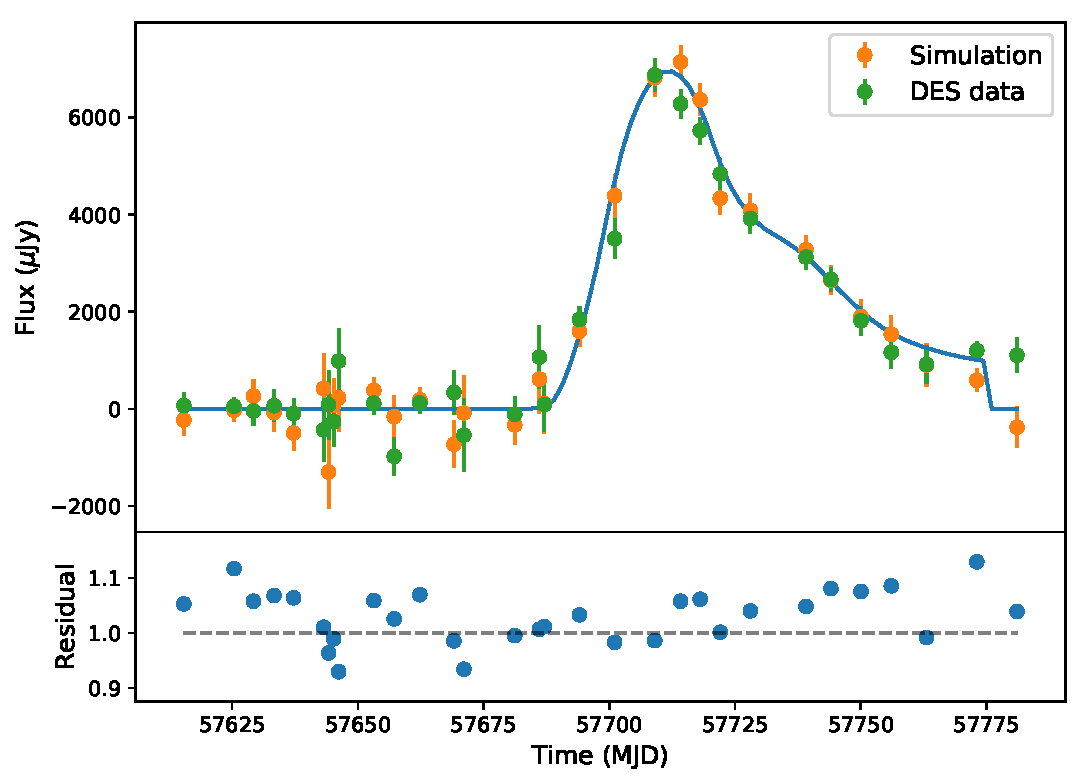
\includegraphics[width=\textwidth]{Figures/Chapter5/IaSim.pdf}
  \caption{\textit{Top}: \textit{r}-band light curve of an example SN\,Ia observed by DES and a simulated object created to replicate the original data point. \textit{Bottom}: the ratio of the S/N for the observed and simulated data light curves shown to be in agreement.}
  \label{fig:IaNoiseComp}
\end{figure}

\subsection{SN\,Ia}
Amongst the various SN classes simulated as part of this thesis, SN\,Ia is unquestionably the most well-studied and understood class of objects. Thanks two decades of use as cosmological probes, there exist a number of packages able to model and simulate these objects with a high accuracy. Furthermore, the parameter spaces of SN\,Ia as well as peculiar outliers to the class (SN\,Ia-91bg and SN\,Ia-91T) are well understood, giving us a firm base on which we can build their simulated samples.

While there are no limiting factors preventing us from performing our own simulations, starting with any implementation of the SALT2 model (e.g SNANA, SNCosmo or otherwise), and passing these through the DES noise model (\sref{sec:NoiseModel}), this would, in essence, replicate the sample of fake SN\,Ia injected into the science images as part of the real-time data reduction pipeline. In DES, these objects are used to estimate the image quality and generate the \textsc{SIMLIB} files making them equivalent to light curve that would be generated through SNANA.

The light curves of SN\,Ia that are injected into the images are generated using the extended SALT2 model as used in \citet{Betoule2014}. The upper redshift range was set as z=1.4 ensuring that the sample is not limited by the simulated redshift. We expect that DES is able to detect SN\,Ia up to redshift z$\sim$1.3. The fake SNe are injected such as to match the rate evolution measured by \citet{Perrett2012}. As a downside of using a predetermined sample of simulated objects, we do not have any control over the number of objects entering it. However, 45,000 objects passing the detection criteria form a sufficiently large sample of SN\,Ia. \fref{fig:IaDist} shows the redshift distribution for our SN\,Ia training set.

\begin{figure}
  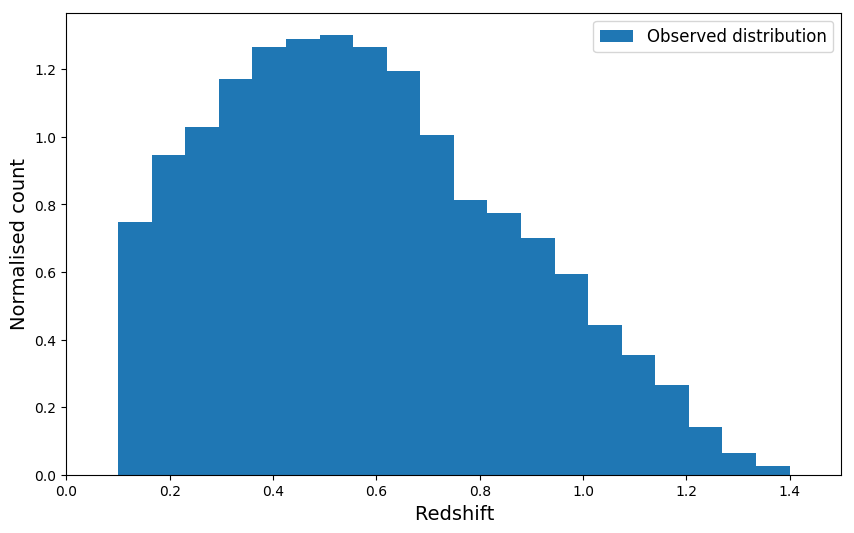
\includegraphics[width=\textwidth]{Figures/Chapter5/SNIa_z_dist.png}
  \caption{The redshift distribution of SN\,Ia that form part of our training sample. }
  \label{fig:IaDist}
\end{figure}

\subsection{Core-collapse Supernovae}
In the local universe, Core-Collapse Supernovae (CCSN) are more numerous than SN\,Ia, with an approximate fraction of 70\% CCSNe to 30\% SN\,Ia  \citep{Alsabti2017}. However, CCSN are a fainter with an average brightness only a tenth of the SN\,Ia luminosity that results in a survey such as DES being able to only detect them up to the z$\sim$0.6 as compared to z$\sim$1.3 for SN\,Ia, giving a much lower observed rate. However note that the training of CNNs requires that each distinct class of objects entering the classification model must be equally represented. We treat hydrigen-rich and stripped envelope CCSNe separately.

\subsubsection{SN\,Ib/c}
In \cref{Chapter3}, I presented \textsc{CoCO}, a method for creating templates as well as simulating SN\,Ib/c, based on the spectroscopic templates shown in \tref{tab:IbcTemplates}. Due to the small number of good spectral templates, the spectral subtypes of the templates do not match their measured relative abundance and, I use the \citet{Li2011} measurement of the local rates of CCSNe to correct their abundances. The decision to follow their observed abundances is based on our lack of interest in subclassifying transients based on their similarity to a specific SN template.

\begin{table}
  \caption{Sample of SN\,Ib/c used within \textsc{CoCo} as template for their class. The variation in the peak luminosity of the SNe results in different upper redshift limit at which the objects are detectable by DES. The SNe with slower evolution and greater luminosity are detected more often in the survey resulting in a higher number of accepted samples.}
  \label{tab:IbcTemplates}
  \centering
  \begin{tabular}{l|r|r}
    SN Name  & redshift & count \\
    \hline
    SN1993J  & 0.79 &  3322  \\
    SN1994I  & 0.70 &   975  \\
    SN1996cb & 0.78 &  2151  \\
    SN1998bw & 0.80 & 16416  \\
    SN2002ap & 0.80 &  2938  \\
    SN2005bf & 0.80 &  8259  \\
    SN2005hg & 0.80 &  1942  \\
    SN2006aj & 0.80 & 11988  \\
    SN2007Y  & 0.57 &   428  \\
    SN2007gr & 0.67 &   954  \\
    SN2007uy & 0.64 &   905  \\
    SN2008D  & 0.28 &   196  \\
    SN2008ax & 0.43 &   766  \\
    SN2008bo & 0.46 &   390  \\
    SN2009iz & 0.80 &  1553  \\
    SN2009jf & 0.80 &  4044  \\
    SN2010al & 0.80 & 14784  \\
    SN2011bm & 0.80 & 24213  \\
    SN2011dh & 0.73 &  2659  \\
    SN2011ei & 0.39 &   410  \\
    SN2012ap & 0.54 &   707
  \end{tabular}
\end{table}

I generate the light curves in the redshift range of 0$<$z$<$0.8, drawn using a volume-weighted, non-uniform random distribution based on the cosmic star formation rate  \citep{Hopkins2006}. To introduce a level of diversity into the sample, I apply host galaxy reddening to the templates (Milky Way extinction is not necessary as DES observed very low extinction fields). I use the \citet{Cardelli1989} law with R$_\mathrm{v}$=3.7 (corresponding to the Milky-way value) and the E(B-V) values drawn randomly from the modulus of a Normal distribution centred at zero with a variance, $\mu$=0.2. I also have used a similar (but unmodulated) distribution to apply an offset to the peak magnitudes of the SNe. This is further aimed at introducing a scatter into the training sample as the low number of available templates, despite being placed at different redshifts and explosion dates, could produce repeating samples of objects that could lead to overfitting.

From the simulations, we measure the detectability of each template as a function of redshift (see \tref{IbcTemplates}) as well as the detection frequency of the whole population as a function of redshift shown in \fref{fig:IbcDist}. As expected SN\,Ib/c are detectable only up to z$\sim$0.8, a distance significantly lower than that of SN\,Ia (\fref{IaDist}).

\begin{figure}
  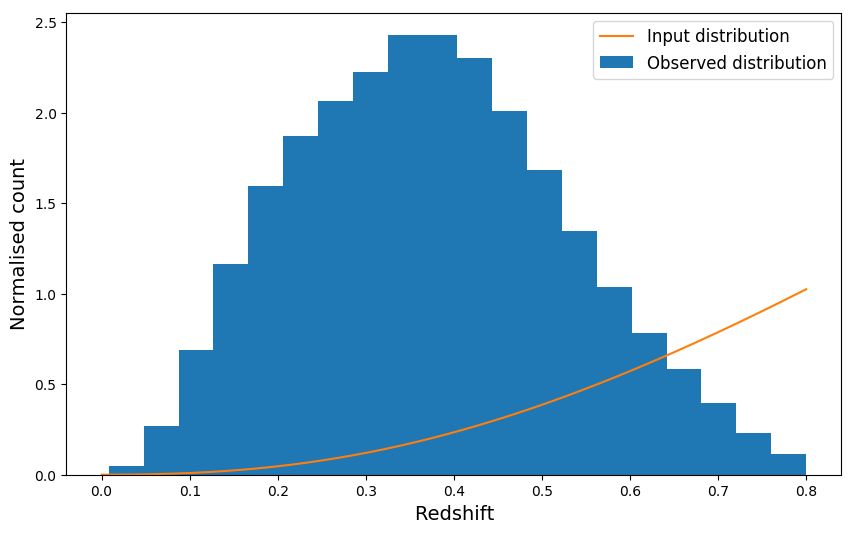
\includegraphics[width=\textwidth]{Figures/Chapter5/SNIbc_z_dist.png}
  \caption{The input distribution of artificially generated SN\,Ibc vs their detection count as a function of redshift. As expected, the detection fraction of SN rises initially with the increase in the volume of the sampled universe before declining at higher redshift due to a decrease in their detectability.}
  \label{fig:IbcDist}
\end{figure}

\subsubsection{Hydrogen-Rich SN}
The method used for building the training sample of SN\,II followed that of SN\,Ib/c. I used the template sample, generated using the \textsc{CoCo} package, in \tref{tab:SNIITemplates}. The only significant difference in the process of generating the sample was the simulated redshift range, which was increased to z$\sim$0.9 as I found during our testing that using z$<$0.8 would result in a number of objects being detected at the upper redshift limit.

\begin{table}
  \caption{Sample of SN\,II used within \textsc{CoCo} as template for their class. This sample is smaller than its sister sample of SN\,Ib/c due to the lower quality of their spectroscopic data.}
  \label{tab:SNIITemplates}
  \centering
  \begin{tabular}{l|r|r}
    SN Name  & redshift & count \\
    \hline
    SN1999el & 0.40 &  4052 \\
    SN2000cb & 0.36 &  4127 \\
    SN2000eo & 0.78 & 20895 \\
    SN2002gd & 0.26 &  1924 \\
    SN2006V  & 0.45 &  7178 \\
    SN2007pk & 0.75 & 18822 \\
    SN2009E  & 0.30 &  3538 \\
    SN2010al & 0.90 & 30882 \\
    SN2011hs & 0.26 &   792 \\
    SN2012ec & 0.36 &  5176 \\
    SN2013ej & 0.36 &  4114 \\
    \hline
  \end{tabular}
\end{table}

\begin{figure}
  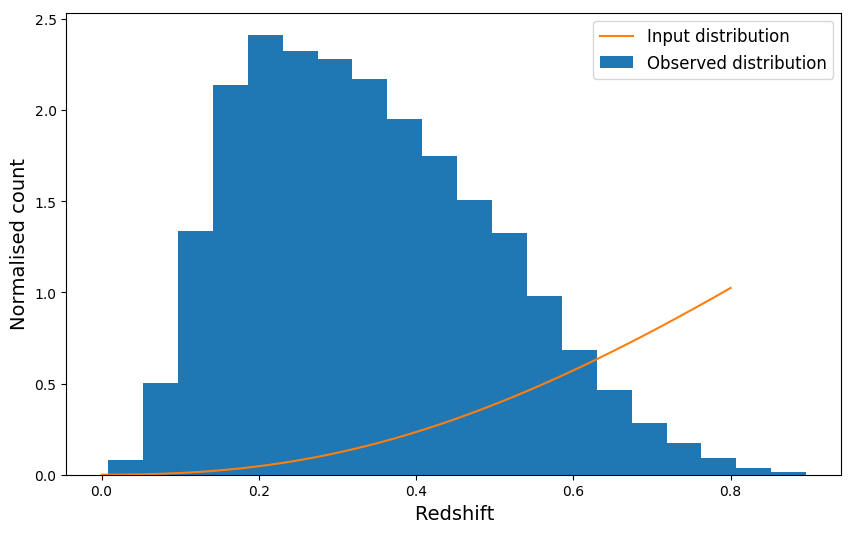
\includegraphics[width=\textwidth]{Figures/Chapter5/SNII_z_dist.png}
  \caption{The input distribution of artificially generated SN\,II vs their detection count as a function of redshift. The distribution is skewed due to the bimodality in the detectability of the training sample shown in \tref{tab:SNIITemplates} thanks to a small number of objects with a much higher intrinsic luminosity than the rest of the sample.}
  \label{fig:IIDist}
\end{figure}

\subsection{SLSN}
The simulations of SLSNe were one of the most challenging topics of this thesis. The low numbers of known examples of this class, combined with the uncertainty surrounding their definition and the engine powering their luminosity makes their modelling a challenging task. For the purpose of a classification study such as the one presented in this thesis, we must not only replicate all previously observed objects but also make a reasonable, but not overly constraining, prediction for what yet unknown SLSNe may appear as and represent as a class. Until recently, this would not have been possible as our understanding of the models of SLSNe and their parameters was not sufficient. However, several works including \cref{Chapter4,Chapter3} of this thesis as well as \citet{Inserra2013,Nicholl2013,Nicholl2017} and Angus et al. (in prep) showed that the spin-down of a Magnetar model is able to provide a good approximation for all SLSNe with an acceptable level of accuracy.

The greatest step towards simulating SLSNe was achieved in \citet{Inserra2018a} where we established a new definition of this class that is versatile and robust enough to produce a sample that matches all observed objects but at the same time is limited in the span such that it does not overlap with other classes of SNe. This definition is based on Four Observables Parameter Space (4OPS), defined in narrow (800\AA~and 1000\AA~wide respectively) box filters centered at 4000\AA~and 5200\AA, by: the peak in the 4000\AA~band light curves, colour between the band at peak and +30 days post maximum, and the drop in magnitude between the peak and +30 days in the 4000\AA~band. \citet{Inserra2018a} finds that SLSNe form linear correlations in this parameter space, with a narrow scatter shown in \fref{fig:4OPS}. I use this property to determine the magnetar model parameters which correspond to the definition of SLSNe.

\begin{figure}
  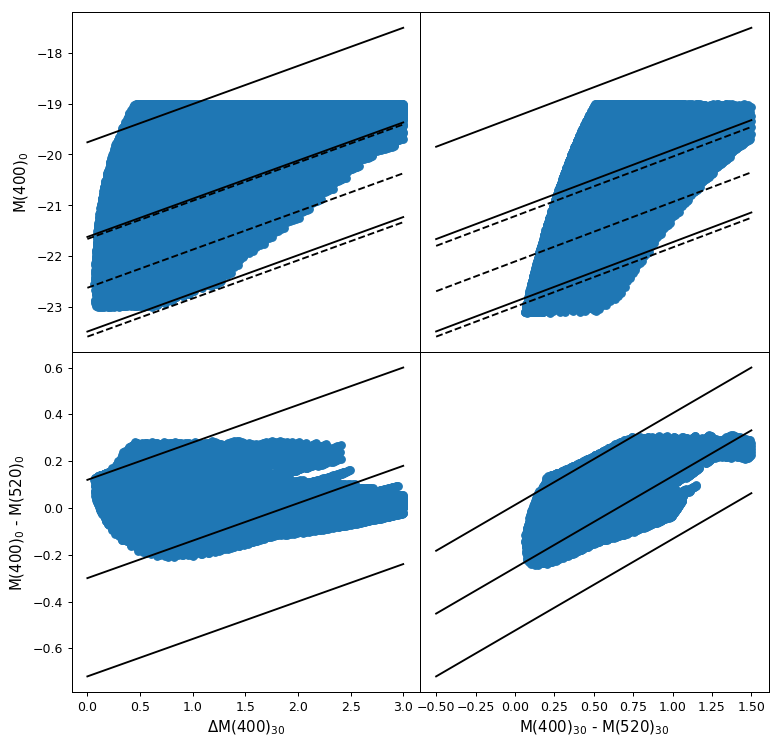
\includegraphics[width=\textwidth]{Figures/Chapter5/4ops.png}
  \caption{The 4OPS parameter space used to identify SLSNe. The solid lines represend the regions used in this work while the dashed lines are the original values found \citet{Inserra2018a}. The shaded area corresponds to the regions where SLSNe, generated using the \textsc{pyMagnetar} pipeline, that are compatible with the 4OPS definition.}
  \label{fig:4OPS}
\end{figure}

I simulate a large number of SLSNe using the magnetar model and compare them to the 4OPS definition. The magnetar model parameters are drawn randomly from a uniform top-hat distribution, bound at 10<$\tau_M<$150, 0.1$<\mathrm{B}_{14}<$20.0, 0.01$<\mathrm{P}_{ms}<$10.0. These limits were informed by the definition of SLSNe used in the rate calculation described in \cref{Chapter4}, but were expanded to ensure completeness and, at the same time, limit the number of computationally expensive simulations that needed to be performed. Furthermore, I introduce a modification to the 4OPS definition of SLSNe, similar to that in Angus et al. (in prep), where the parameter spaces are expanded by one magnitude of scattering while retaining the original slope of their relationship. This was aimed at including fainter objects such as those found in the DES spectroscopically confirmed sample (\sref{sec:DES_SLSN}), that were not available at the time the relationship was constructed. The modified limits are presented in \tref{tab:4OPS} and can be seen in \fref{fig:4OPS} along with the regions where objects drawn from the magnetar model.

\begin{table}
  \caption{Definition of borders in the parameter space of 4OPS defining SLSNe in this thesis. The line represent the enter of the defining region which is constrained by within the 3$\sigma$ confidence region parallel to the line.}
  \label{tab:4OPS}
  \begin{tabular}{c|c|r|r|r}
    x-Axis & y-Axis & Intercept & Gradient & 1$\sigma$ \\
    \hline
    $\Delta$M(400)$_{30}$ & M(400)$_0$ & -21.62 & 0.75 & 0.62 \\
    $\Delta$M(400)$_{30}$ & M(400)$_0$ - M(520)$_0$ & -21.02 & 1.14 & 0.59 \\
    M(400)$_{30}$ - M(520)$_{30}$ & M(400)$_0$ & -0.3 & 0.16 & 0.14 \\
    M(400)$_{30}$ - M(520)$_{30}$ & M(400)$_0$ - M(520)$_0$ & -0.22 & 0.35 & 0.08
  \end{tabular}
\end{table}

\begin{figure}
  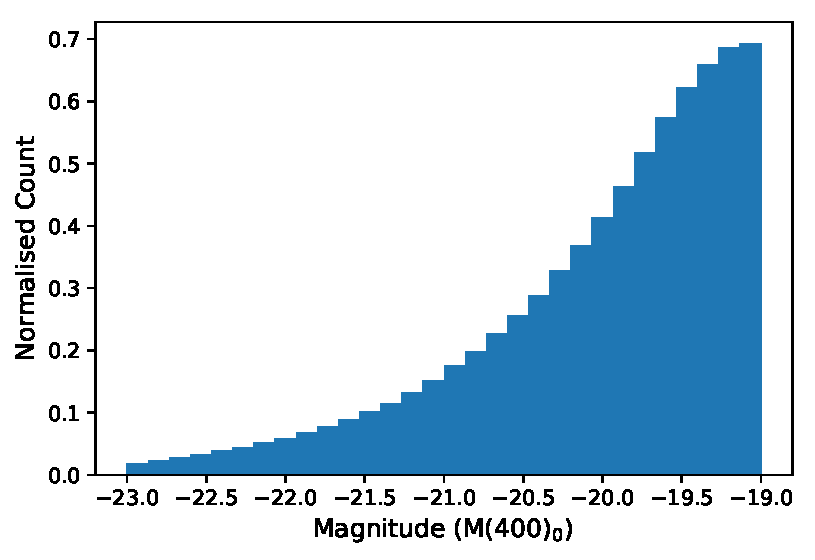
\includegraphics[width=\textwidth]{Figures/Chapter5/MagDist}
  \caption{Distribution of peak magnitudes for SLSN generated using \textsc{pyMagnetar}. The parameters used to generate the light curves have been drawn uniformly from the magnetar model parameters space and were first compared to the 4OPS selection criteria before being used.}
  \label{fig:4OPSParams}
\end{figure}

\begin{figure}
  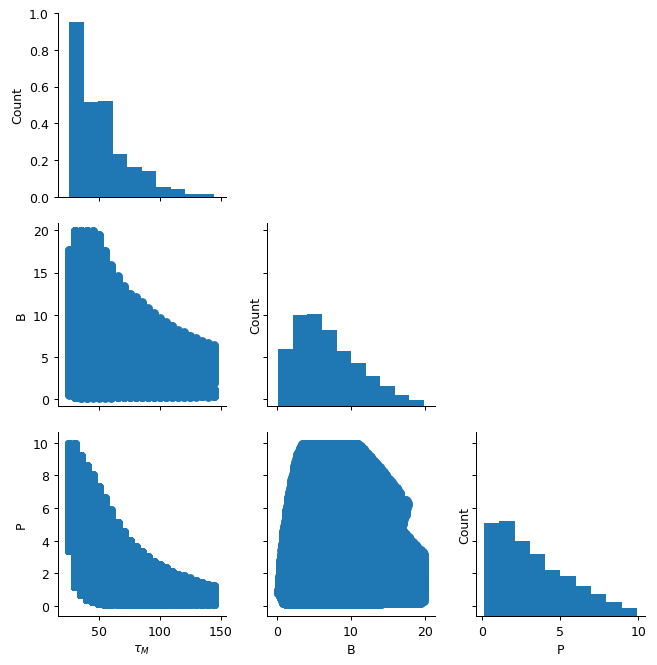
\includegraphics[width=\textwidth]{Figures/Chapter5/MagParams.png}
  \caption{Distribution of magnitudes model paramaters that result in a SLSN-like event that matches their 4OPS definition \citep{Inserra2018a}.}
  \label{fig:4OPSMag}
\end{figure}

In \fref{fig:4OPSParams}, I show the distribution of magnetar model parameters that produce objects that match the 4OPS definition of SLSNe. Perhaps the most interesting result is the luminosity function that results from uniformly drawing objects from the magnetar model parameter space, shown in \fref{fig:4OPSMag}. With no external inputs, the function matches that observed by \citet{DeCia2017} in the PTF sample of SLSNe, showing a rapid increase in the number of fainter objects. I use the sets of magnetar model parameters that match the SLSN definition to generate their training sample. In total, $\sim$100,000 SLSN were generated at a range redshifts with 0$<$z$<$3, drawn from a volume-weighted distribution following the SFR of the universe \citep{Beacon2004} similarly to that used for simulating CCSNe (\fref{fig:SLSNDist}).

\begin{figure}
  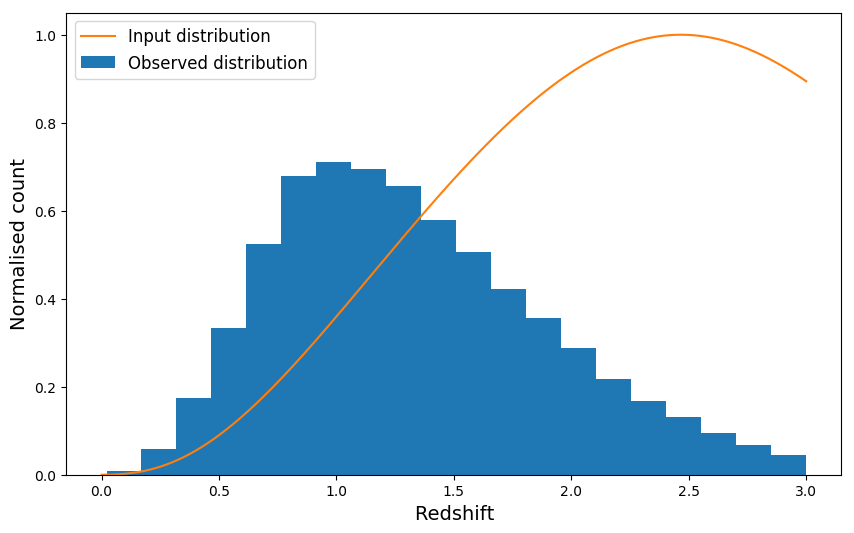
\includegraphics[width=\textwidth]{Figures/Chapter5/SLSN_z_dist.png}
  \caption{The input distribution of artificially generated SLSN vs their detection count as a function of redshift. The superior luminosity of these objects compared to other CCSNe is apparent when comparing their detectability ranges. This also motivates further our search as we know that DES should be able to detect SLSN up to z$\sim$3, while the most distant object to date was confirmed at z=2.0}
  \label{fig:SLSNDist}
\end{figure}

\subsection{AGN}
Active Galactic Nuclei (AGN) are the largest contaminant in the DES transient sample. This is partially due to their physical morphology and, in greater measure, the design of the survey. AGNs are most commonly associated with long, quasi-periodic, variable light curves that are often easy to identify based on their historical variability. As no long-term observations, matching its depth, are available for the DES SN fields making each first AGN detection its discovery. Prior to the first season of DES, a set of science verification images were taken as templates for the image subtraction pipeline used to detect new transients. AGNs that have undergone rebrightening in the first season were detected as potential supernova candidates. If the templates remained unchanged for the duration of the survey we would see a decrease in the contamination each season. Furthermore, we would be able to remove most of these transients retrospectively by selecting objects with detections in multiple seasons. The survey did, however, change the templates each year in the first three seasons of its operations to increase the quality of the images used as templates. In the final two seasons, the data from Y2 was used as templates. Additionally, the data for the first season was also later reanalysed using Y2 images as a template. A caveat of DES that caused us particular issues is that negative `detections' are not considered as detections within the transient selection algorithms. As a result, each DES season contains a large number of objects which are selected as new transients despite showing strong visual signs of prior, albeit `negative', variability.

In the cases of SLSNe, this is particularly troubling as their slow evolution can be sometimes confused with an AGN with a quasi-period of approximately one year if only single DES seasons are considered. It is, therefore, imperative that AGNs are correctly represented in the ML training sample used in \sref{sec:CNN}. For this purpose, I use the existing simulations of AGNs, in the DES observing bands, presented in \citet{Honig2016}. While these simulations were originally aimed at evaluating the possibility of using AGNs as cosmological probes, using a technique referred to as Reverberation Mapping, they were suited perfectly for this project. The simulated light curves did not include any survey noise, were densely sampled (one-day cadence) and had a span exceeding four years. In total 100,000 simulated objects were available for this study including those placed at redshifts outside the detectable range for DES. I have therefore placed each object at random start dates and fields, before applying the survey noise using the method described in \sref{sec:NoiseModel}, resulting in $\sim$60,000 detected AGNs.

\subsection{Noise}
Visual inspection of the DES light curve data shows that a limited number of objects, originally recognised as a real transient according to the DES transient selection criteria (\cref{Chapter2}), do not appear to be physical in origin. There appear to be two main origins for these objects: bad image subtractions and spurious noise detections. Despite a sophisticated, ML powered, transient selection pipeline \citep{Goldstein2015}, some objects (often elongated and with negative subtractions; \fref{fig:BadSubtractions}) can pass the ML cuts, albeit with a low score. In some cases, likely dependant on the observing conditions, this may occur in several epochs separated by less than 30 days, giving the object a `real transient' flag.

Another channel that can result in the misclassifications of candidates is the detection of slow-moving, near earth object. Such objects are most commonly detected at the same position only in two or three consecutive bands. In subsequent epochs, they are, in normal circumstances, no longer detected at the same position resulting in the object being rejected. However, in some rare cases, bad subtractions or random noise spikes exceeding the 5 sigma detection limit, within 30 days cut can result in a `real transient' flag.

\begin{figure}
  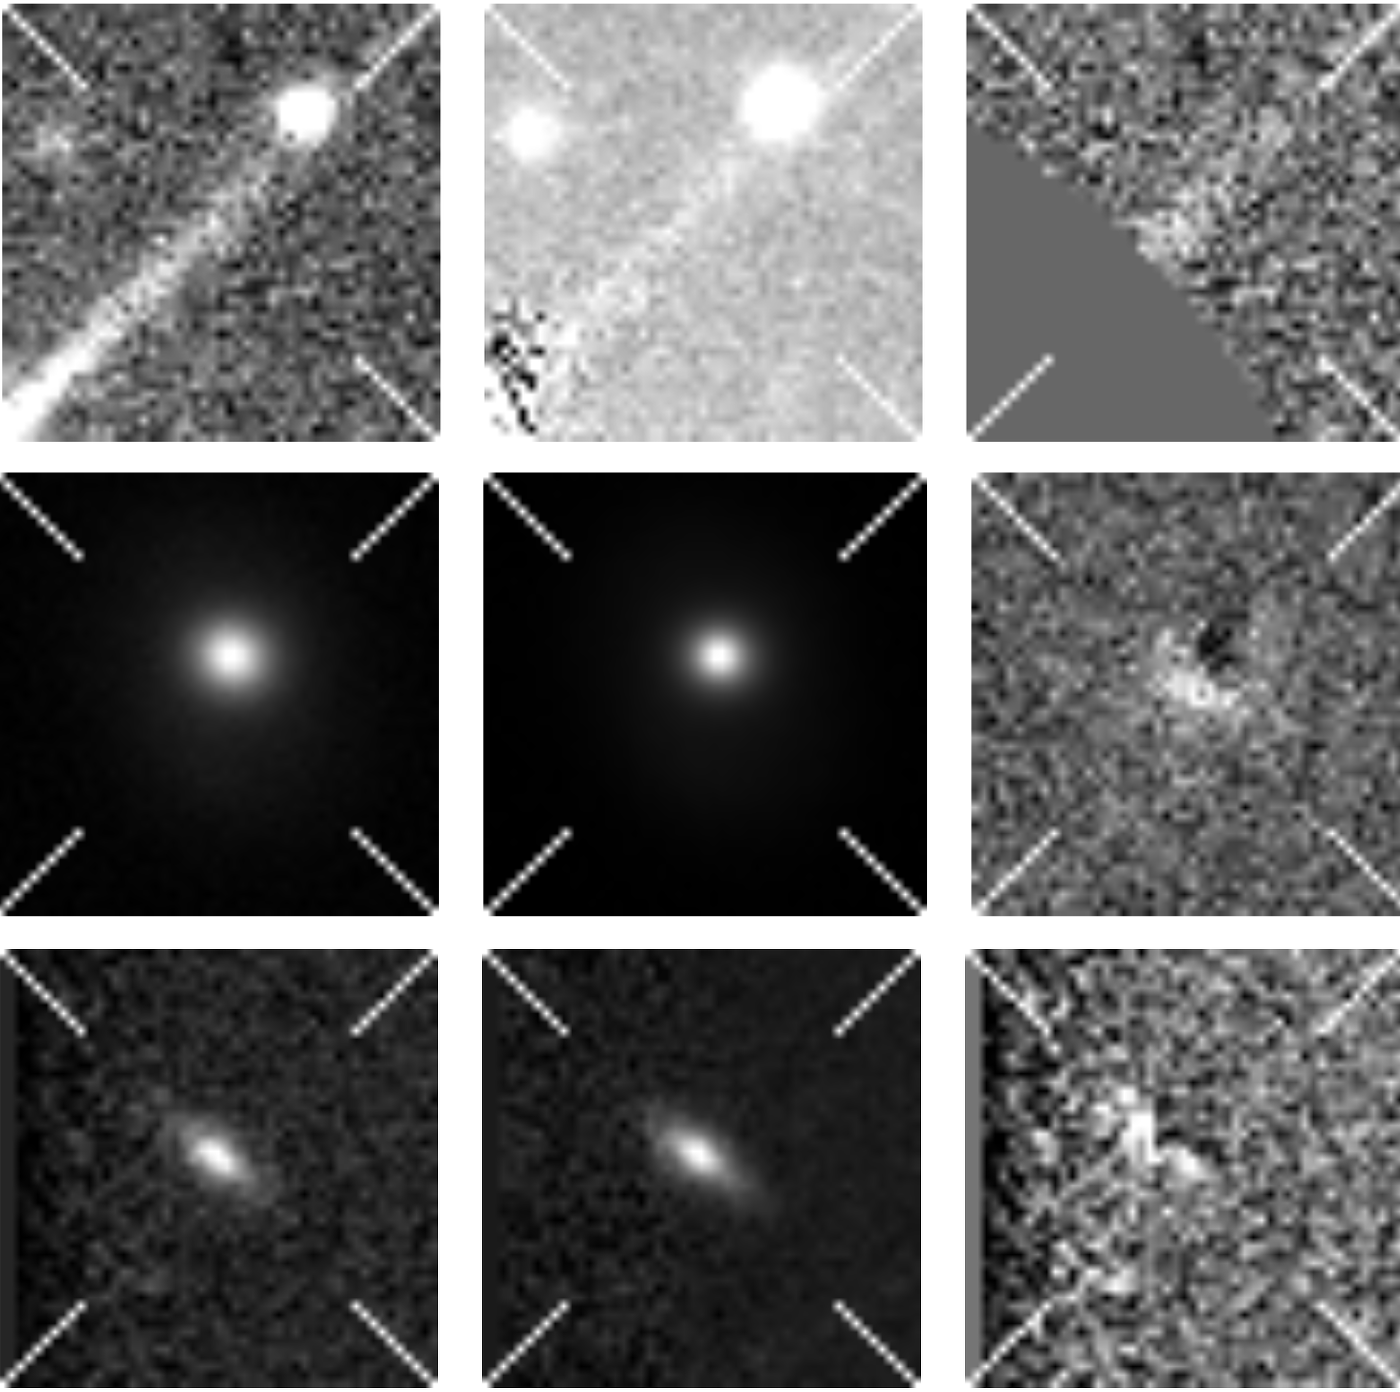
\includegraphics[width=\textwidth]{Figures/Chapter5/BabSubs.png}
  \caption{Examples of bad subractions of DES images. \textit{Left} shows the science images, \textit{center} represent the image subractions templates and on the \textit{right} are the subracted images showing defects.}
  \label{fig:BadSubtractions}
\end{figure}

To model these objects, I use a very simple approach of inserting a number of sharp, $\delta$-function like spikes in the data that correlate between the filters and are separated by less than 30 days to account for the misidentifications. The spikes are selected between 19$<$mag$<$22 in order to test the different behaviours of the GP interpolations used in the next step of this analysis (\sref{sec:DataAugmentation}). The absolute value of the peak does not play an important role in the classification process as the data is normalised before entering the CNN. Similarly to other classes of transients, $\sim$100,000 objects have been simulated across all fields.

\subsection{Missing classes}
While in this thesis, I have created one of the most thorough training samples of SNe for the purpose of a ML classification study, it still cannot be said to be complete. There are a number of classes of known transient objects which I was unable to account for in this work. Some objects such as kilonovae, associated with gravitational waves as their optical counterparts, evolve too rapidly to be using the cadence of DES. Omitting these (undetectable) events does not bring any difference to the final result of our classification. However, one class of objects which could have an effect on our final classification are the newly discovered class of rapidly evolving SNe \cite{Drout2014,Kepler2018}. Recent work by \citet{Pursiainen2018} showed that these objects are relatively common within DES with 72 detections in the first four seasons of its operations. While there are now early, tentative signs \citep{Pursiainen2018} that these objects are powered by a SN shock interacting within a thick an extended wind \citep{Piro2015}, similar to the model used in modelling of the `bumps' found in SLSNe \sref{sec:MagExtensions}. It is this particular connection that would be interesting to explore, however, the modelling of these objects is still in its infancy. The model parameter spaces defining them, their SED models and other similar aspects developed for SLSNe over the last several years have not yet been studied for these fast-evolving SNe.

The omission of rapidly evolving SNe from our sample will result in these objects being mislabelled in our classifications. It would, however, be unlikely that any of the objects that we have not included in the training sample would get mislabelled as a SLSNe due to their significantly faster evolution. I test this assertion in \cref{Chapter6} using the ground-truth sample of objects identified by \citet{Pursiainen2018}.

\section{Data Augmentation} \label{sec:DataAugmentation}
Before the training sample of SNe created in \sref{sec:TrainingSample} can be used to build a CNN classification model, it has to first undergo a number of augmentation steps. The data passed through the CNN must be uniform in terms of the number of data points as well as their separation, regardless of the field and season the data originated from. To achieve this, I must first select a suitable length of observations and cadence that overlaps the most closely with that observed by DES. Furthermore, I apply a flux correction required to normalise the effect of using a varying subtraction template in a different season. Finally, I use GPR to interpolate and augment the data such as to meet the requirements of CNN.

\subsection{Choosing the observing block} \label{sec:ObsBlock}
I define the observing block, for the use in our classification study, as the span of time (measured in days) that is the longest period over which all DES seasons observe all of its fields. Due to the observing conditions and scheduling, the DES observing periods vary between the seasons and fields. The difference between the longest and shortest observing window in DES measures 40 days.

Selecting the observing block is more complex than simply selecting the length of the shortest season. \fref{fig:ObsBlock1,fig:ObsBlock2,fig:ObsBlock3,fig:ObsBlock4} show the cadence of DES in Y1-4 in all fields and bands. Instead, this is done in two stages: first I find the span that covers all the filters: from the first point where all the filters are observed, to the last point where all the filters are observed. I then remove the points at the beginning of the season in cases where the gap in the data is longer than 10 days. This is a common consequence of observations being missed due to the atmospheric conditions. Data does not have to be similarly removed at later stages of the light curve as the GPR interpolation can account for large gaps as long as they are supported by a number of points either side of the intermission.

From these measurements, I determine the optimal observing block to be 149 days in duration. The span covered by the block in each season and filter is shown in \fref{fig:ObsBlock1,fig:ObsBlock2,fig:ObsBlock3,fig:ObsBlock4}. Due to the improved quality of the light curves in the second part of each season, I place the observing block as late in time as possible.

\begin{figure}[h]
  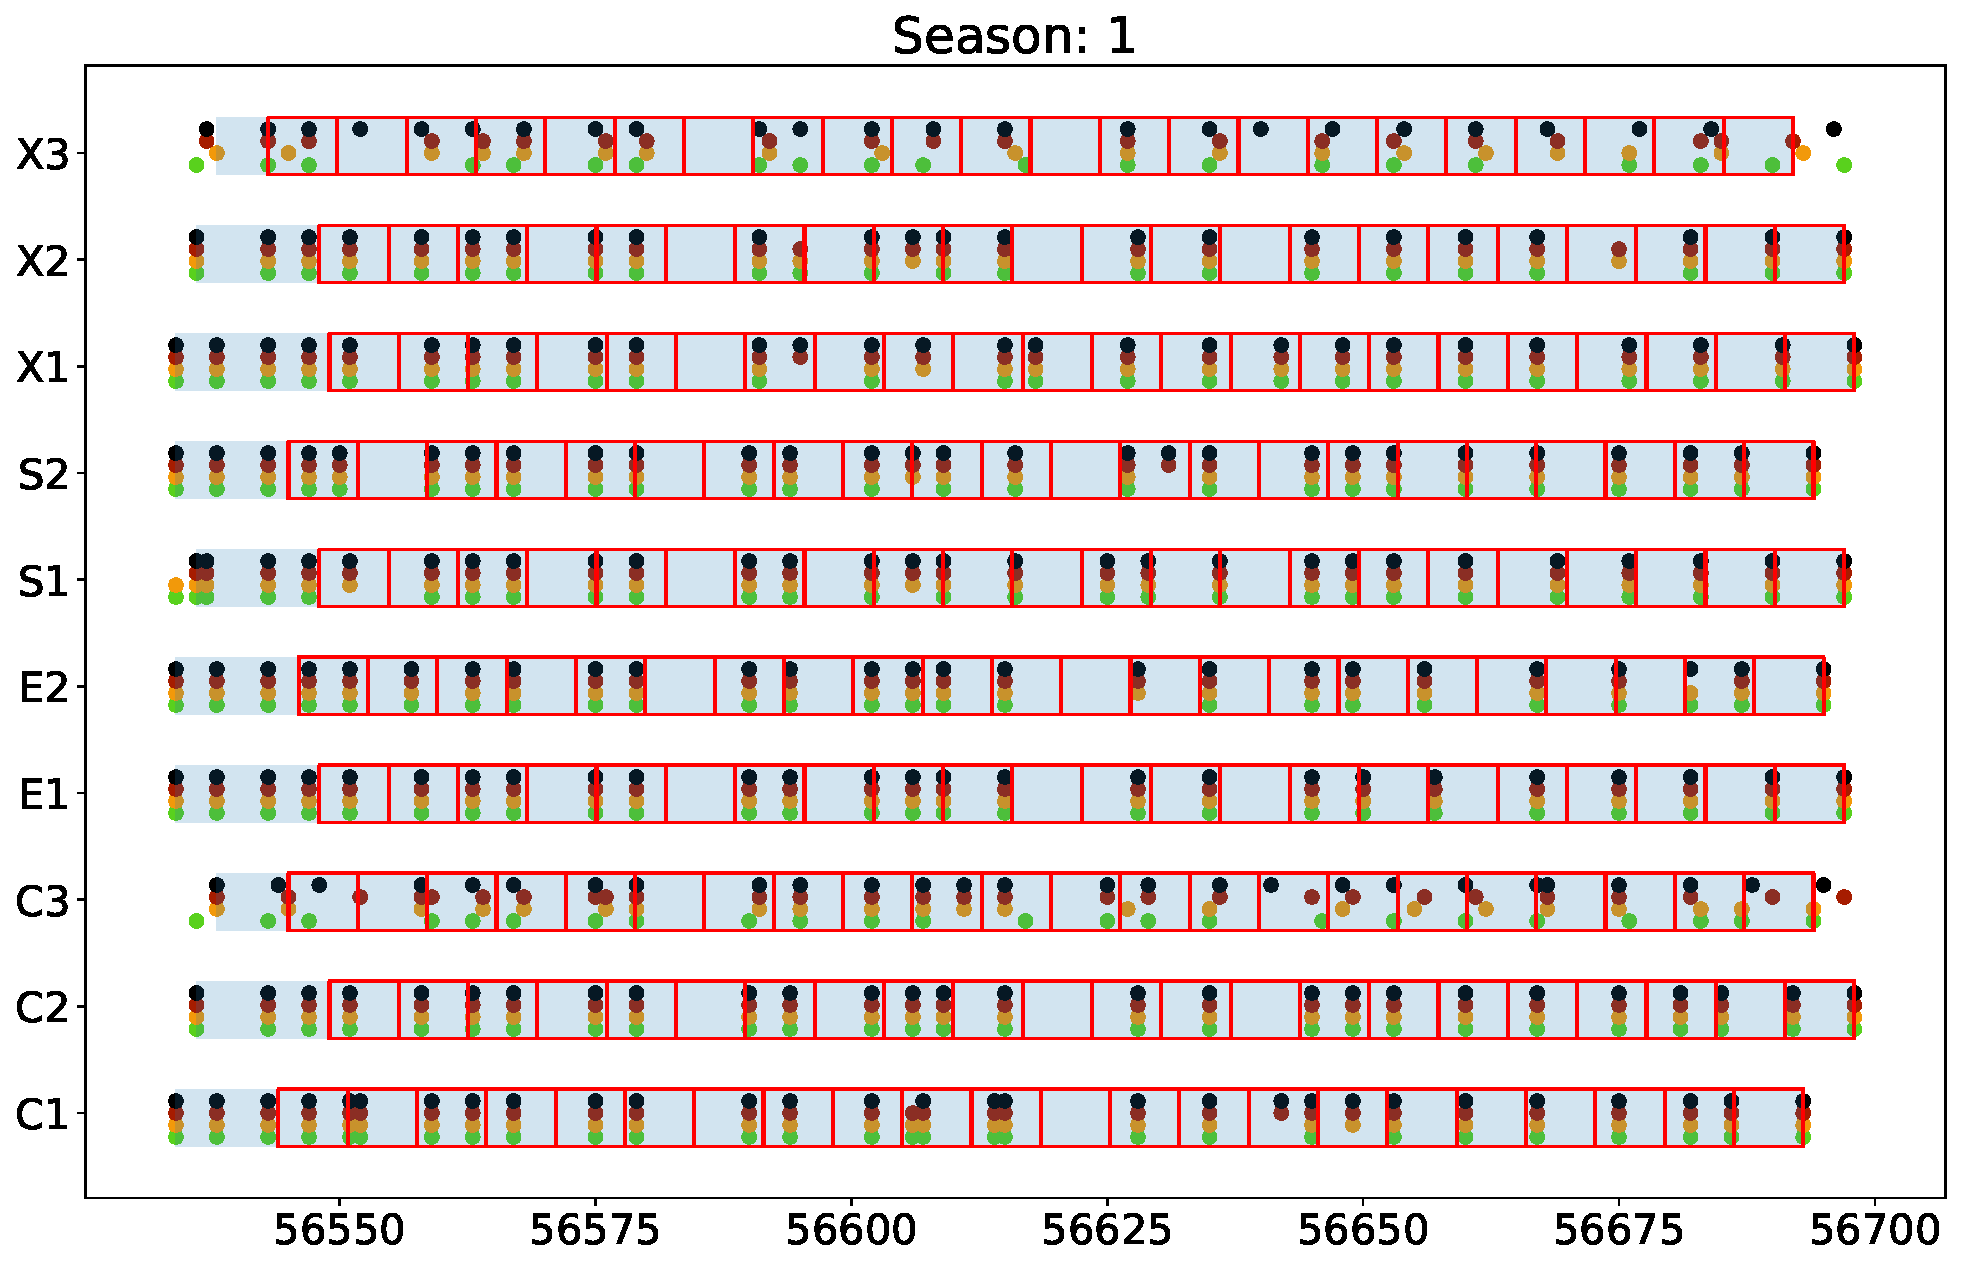
\includegraphics[width=\textwidth]{Figures/Chapter5/ObsBlock_Season1.pdf}
  \caption{The cadance and observing block of the first season of DES}
  \label{fig:ObsBlock1}
\end{figure}

\begin{figure}[h]
  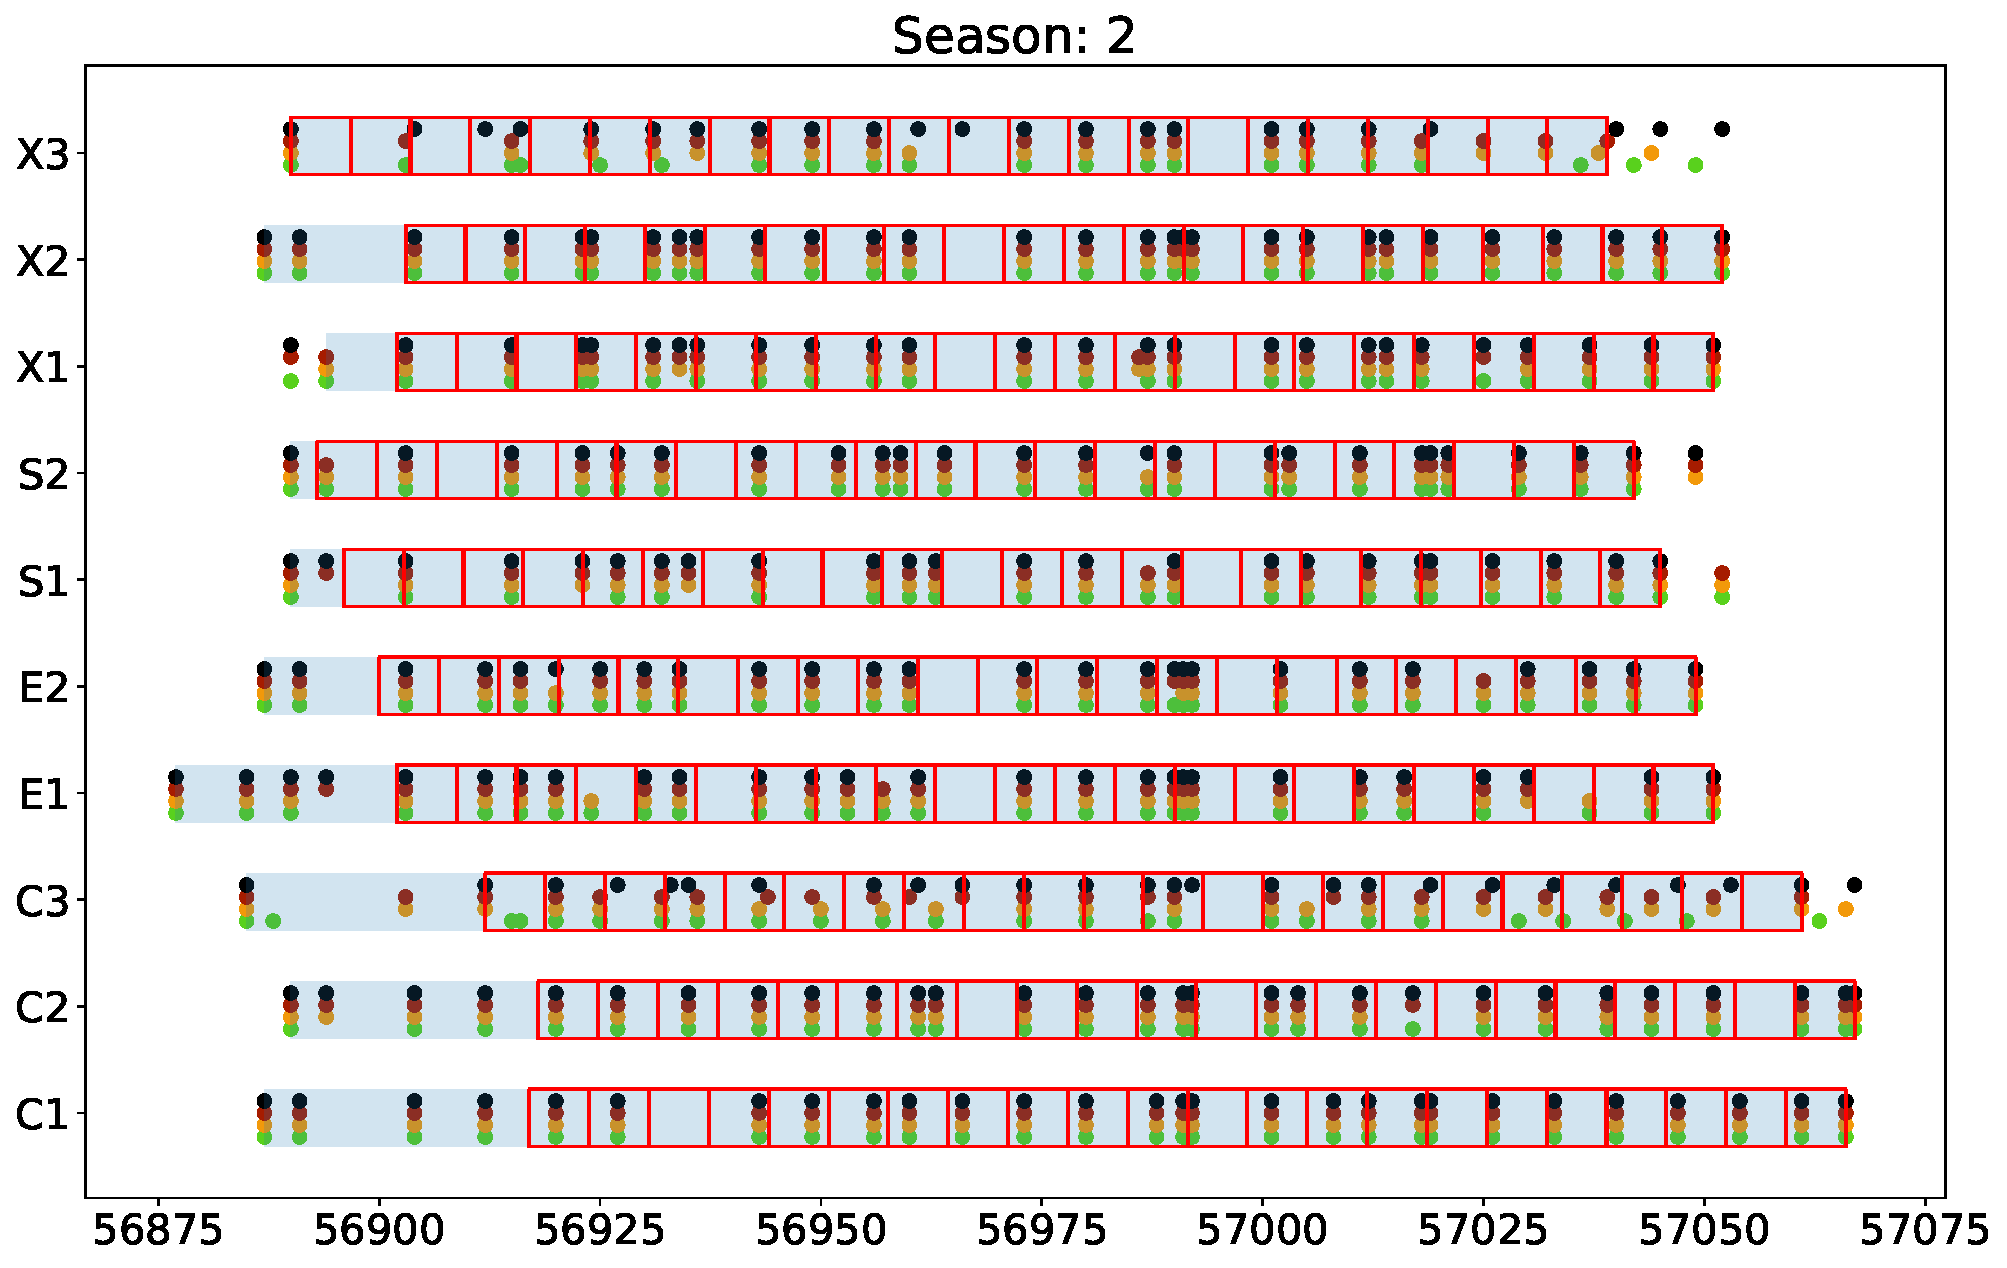
\includegraphics[width=\textwidth]{Figures/Chapter5/ObsBlock_Season2.pdf}
  \caption{The cadance and observing block of the secon season of DES}
  \label{fig:ObsBlock2}
\end{figure}

\begin{figure}[h]
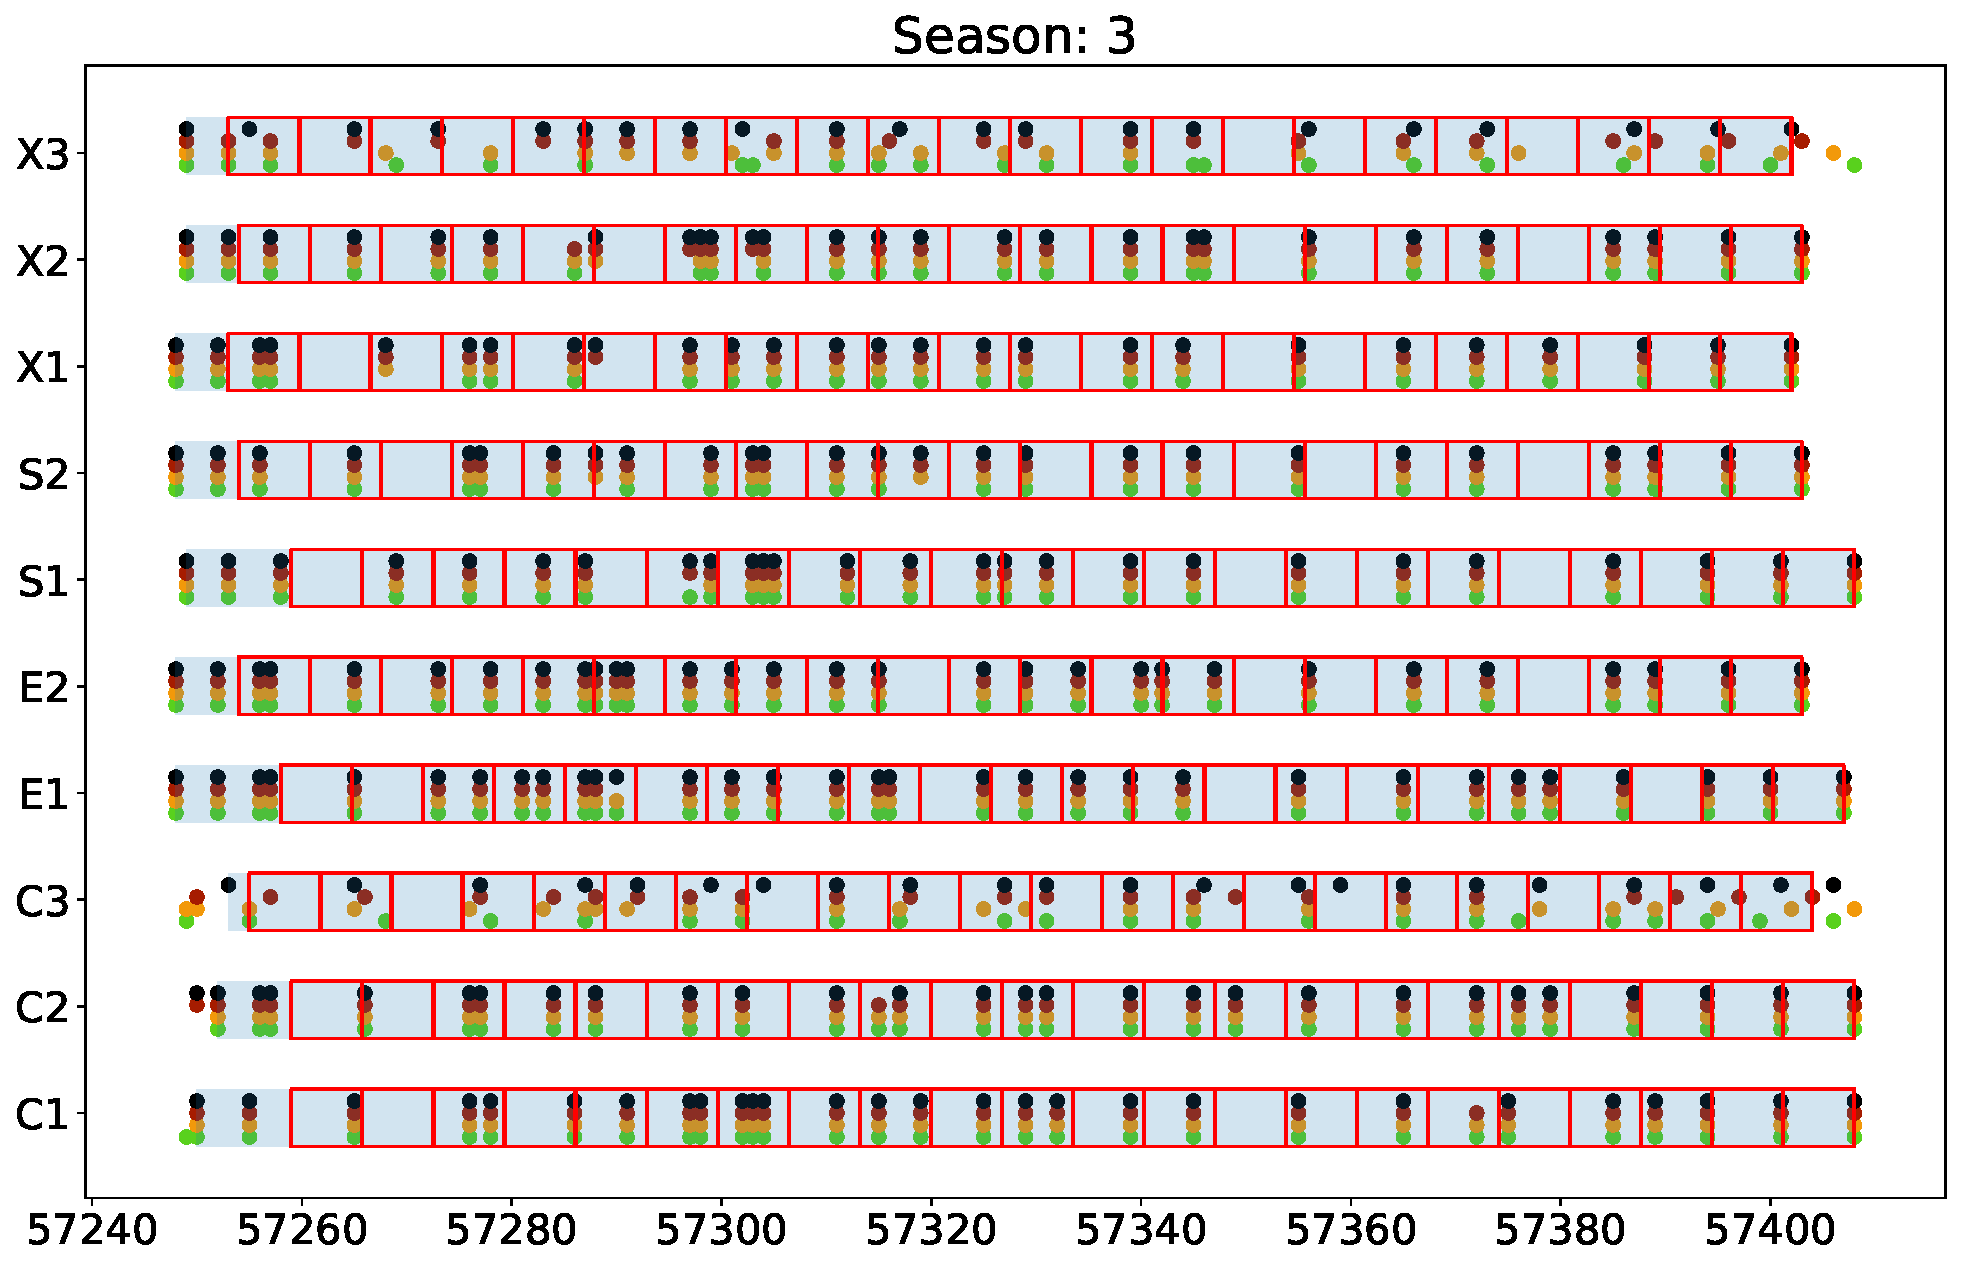
\includegraphics[width=\textwidth]{Figures/Chapter5/ObsBlock_Season3.pdf}
  \caption{The cadance and observing block of the third season of DES}
  \label{fig:ObsBlock3}
\end{figure}

\begin{figure}[h]
  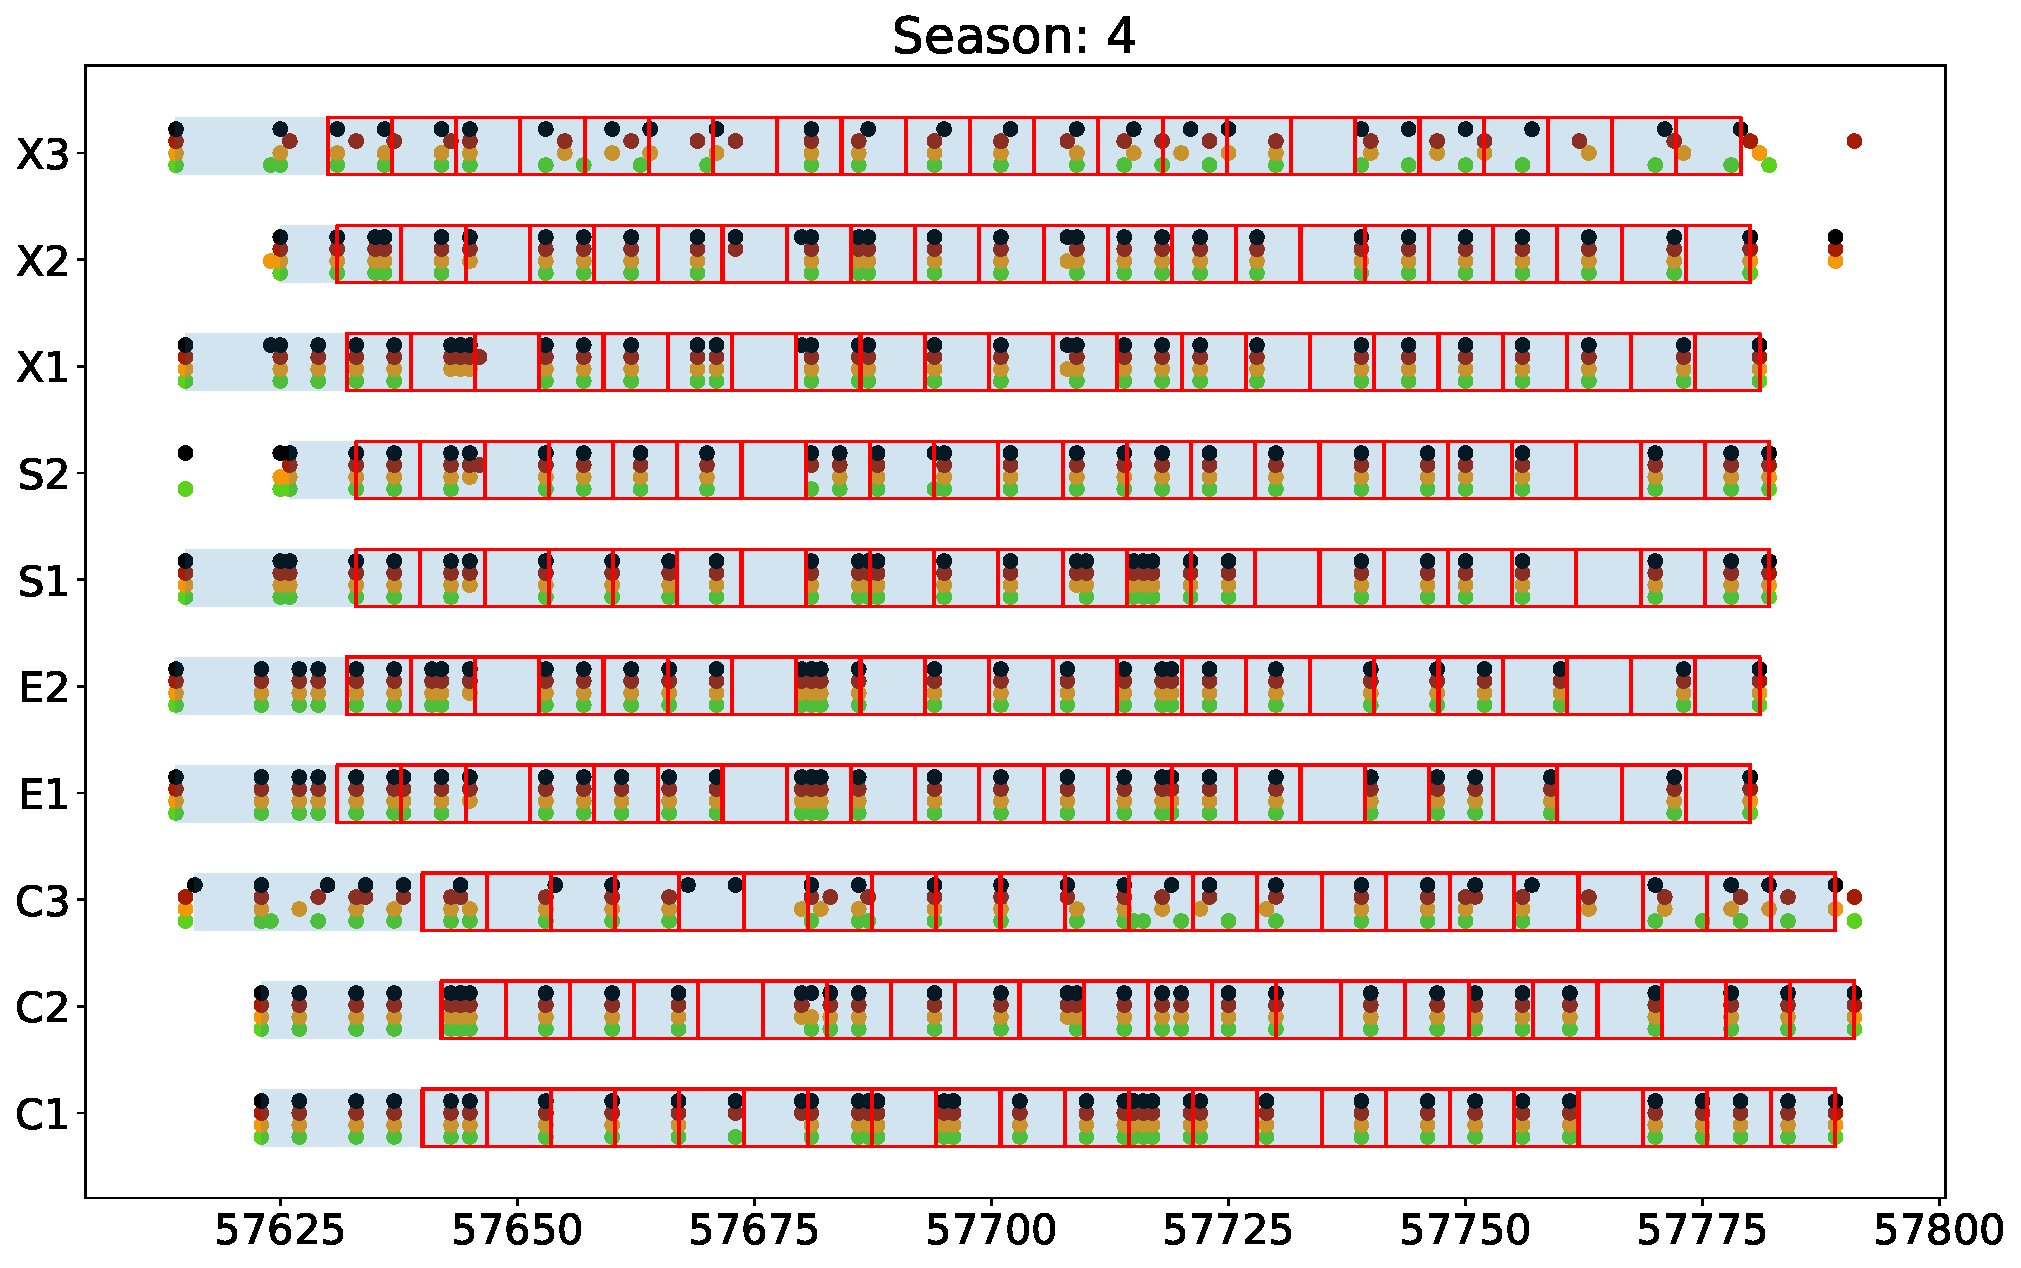
\includegraphics[width=\textwidth]{Figures/Chapter5/ObsBlock_Season4.pdf}
  \caption{The cadance and observing block of the forth season of DES}
  \label{fig:ObsBlock4}
\end{figure}

\subsection{Choosing the cadence} \label{sec:SimCadance}
Upon deciding the length of the observing block used in the simulations, the next step is to choose the cadence of the interpolated observations. As GPRs are used to augment the data, essentially any cadence can be used. As there are no rules or precedences set out in the literature that discuss the optimum treatment of the augmented data, I must make an informed decision. The factors which balance the decision is on one side to represent the data without the loss of any information observed by the survey, while at the same time not introducing too many points which, essentially, duplicate the information.

The observed cadence of DES is not uniform and varies through the season due to the observing conditions. Early in the season, the cadence is shorter as the observing weather conditions don't allow for the observations of the wide DES fields leading to a shorter DES cadence as the deep and shallow fields are given more observing time. On the opposing end, the cadence stabilised as the season progresses and settles at the designed 7 days. This is seen in \fref{fig:cadence} resulting in a bimodal distribution with an average cadence of 5 days. With a lack of any other factors, I use this value as the base for the cadence used in \sref{sec:UseGP}.

\begin{figure}
  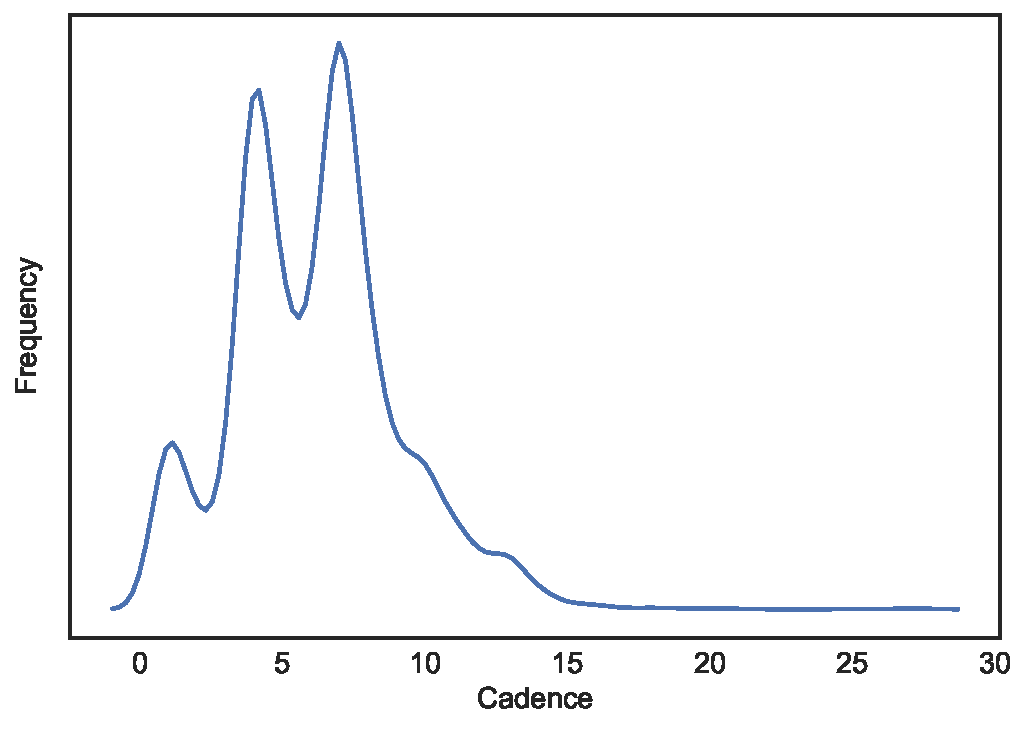
\includegraphics[width=\textwidth]{Figures/Chapter5/Cadence.pdf}
  \caption{Kernel Density Estimate (KDE) plot showing the cadence of DES across all seasons, field and bands. The bi-modality of the distribution can be attributed to the balance between the designed DES cadence of 7 days, occurring only in the perfect conditions, and the actual cadence of 3 days observed in the early parts of each season.}
  \label{fig:cadence}
\end{figure}

\subsection{Applying Flux correction to Real Data}
Before the GPR can be applied to the data, a final correction is the effect of DES exchanging the image subtraction template between seasons. As the focus of the DES SN team is predominantly the study of SN\,Ia, the decision was made to maximise the quality of single-season light curves. As the image quality improved throughout the initial two seasons of observations, the templates have been updated each year. While optimal for the study of short transients, where only a single season is of interest, for slowly evolving SNe (and AGNs) this causes an issue where the supernova light curve is present in the template resulting in decreased flux in the subsequent season. This is a particular problem for SLSN, where their evolution can often be slow enough to be detectable in multiple seasons in DES (Angus et al.; in prep). This could potentially be a factor leading to the misclassification of SLSNe and hence cannot be ignored.

While the optimal approach to this would be to perform the image subtraction and source detection with a single template, this would be computationally prohibitive due to the scale and complexity of the raw DES data. As an alternative, I used the DES analysis logs to determine the observations that have been used in the creation of the template images. In these frames, I measure the median flux of the object and use this value to correct the offset. As a simple test for this approach, I use a light curve of a SN\,Ia that exploded early in the second season of DES. In the uncorrected DES light curves, this results in a flat but negative light curve in the third season.

\subsection{Applying GPs} \label{sec:UseGP}
The size and extent of the training sample used in this thesis are one of the two advancements made towards classifying SNe in DES using the ML approach. An equally important step, crucial for the use of CNNs, was the use of GPR (\sref{sec:GP}) as a tool for light curve interpolation and augmentation. CNN performs pattern recognition using a set of convolutional kernels with a fixed size, therefore requiring the data to be evenly sampled. This has tremendous benefits as it does not require any feature extraction steps and uses every data point in the classification process. While the observed data cannot be used directly with this technique due to its non-uniform sampling, using a GP interpolated light curves removes less information about the data than a parametric model. Simultaneously, it does not introduce any correlations between the distinct bands, both in terms of the flux and the onset of the SN.

I apply the method described in \sref{sec:GP} to interpolate the light curves using the Mate\'rn 3/2 covariance functions. I perform the interpolation over the period selected in \sref{sec:ObsBlock} using the base cadence found in \sref{sec:SimCadance}. After testing the CNN in \sref{sec:CNN}, I found that using a cadence which doubles the original 5 days, to 2.5 days, improves the accuracy of the model. The motivation behind the doubling of the cadence was to allow a gradient for each point to be calculated closer to the point itself as opposed to between the points. The extra points act as control points in this scenario.

\section{Classifications} \label{sec:CNN}
The construction of the artificial DES training sample of transients was a major step towards performing their comprehensive classification study using the ML approach. In recent years, the use of ML expanded far beyond the purely academic uses within the field of Computer Science. The world around us is currently being shaped by Artificial Intelligence (AI) augmented technologies, driven in large measure by Artificial Neural Networks (ANN) and their derivatives such as Convolutional Neural Networks (CNN) and Deep Learning.

The process of selecting transients for spectroscopic follow-up is an example, albeit not explicit, of SN photometric classification. This task has been performed manually, via the visual inspection of the light curves, for decades in every SN survey. In recent years a number of attempts have been made to devise a pipeline for photometric classification of SN based on the clustering of light curve model parameters. However, this problem can be approached from a more fundamental point of view using AI. Computer vision, a prominent branch of AI, has been successfully applied to countless examples of classification tasks where humans demonstrated a superiority over the early classification methods. Projects such as ImageNet \citep{Russakovsky2014} were able to produce models capable of identifying a number of everyday entities (humans, vehicles, animals, household items) with an accuracy exceeding that of an average human. While the scarcity of the training samples available to us in comparison to projects such as ImageNet does not allow us to use an equally complex model, this is not required as the complexity and diversity of our transient data is not as high as that of an everyday object.

In this section, I describe the use of Convolutional Neural Networks (CNN) as an AI tool used to first identify SN light curves in the DES data and subsequently classify them into their respective subclasses with the overall aim of producing a photometric sample of DES SLSNe.

\subsection{Convolutional Neural Networks} \label{sec:CNN}
CNNs are currently one of the hottest topics in the world of AI and ML. While their widespread use is novel and a result of the increase in the performance of computer devices, the theory behind them dates back to the early work on Artificial Neural Networks \citep[ANN;][]{Mcculloch1943} and replicating the of humans ability to learn from an external stimuli.

\subsubsection{Artificial Neural Networks}
All principal components of an ANN are fundamentally based on the human brain contain neurons, represented by nodes and activation functions. The nodes, usually arranged in a network of layers, are connected by a set of weight that corresponds to the biological synapsis. The aim of an ANN is to perform a non-linear transformation between the input parameters and the output values.

ANN is formed through a network of fully interconnected layers, containing activations functions that, in essence, calculates the weighted sum of the inputs and creates an output that acts as an input for the next layer. The choice of activation functions is extremely important to the performance of an ANN. The most commonly used form; the sigmoid function produces an output near to one for inputs that are accepted and zero for the rejected values. The Rectified Linear Unit (ReLU), another commonly used activation function, acts in a similar way but produces a linear output that tends towards infinity above a certain activation value.

The choice of the number of layers is dictated by the complexity of the problem tackled by the network. Between the input and output layers lays a number of hidden layers. While the input later must match in size the dimensions of the input dataset and the dimensions of the output later must match the number of individual classes present in the training set, the hidden layers can have an arbitrary shape. The process through which the networks calculate the weights is referred to as Backpropagation which performs a form of a stochastic gradient descent to optimise the loss (or residual) function. There is numerous implementation of the loss functions and backpropagation algorithms, however, in this work, I chose to use the defaults found in the TensorFlow package: `cross-entropy' and `Adam' respectively.

\subsubsection{Convolutional Neural Networks}
Convolutional Neural Networks (CNN) is a type of Deep ANNs where at least one layer is a convolutional layer. These layers are designed to work similarly to edge and shape enhancing features found in popular image processing software, but instead of relying on predetermined forms learn to best match the structure of the objects found in the training sample. An important feature of CNNs is additional Pooling layers which extract the enhance information from the convolved data through a process of dimensionality reduction. The most commonly used Max Pooling layer works by passing a sliding window, of length $n$, over the data convolved with the filters, with length $m$, and selecting the highest valued pixel to create new output data with length $n-m+1$

\subsection{SNe vs AGN vs Noise}
While CNNs are extremely powerful in their ability to classify images, regardless of what they contain, they often rely on huge training samples in order to learn their discriminating features. In the case of DES transient data, we are still not operating on a sufficiently large dataset despite the work on enhancing the sample. However, it is possible to simplify the classification problem to reduce the number of training samples required to produce a good classification score.

\subsubsection{Choosing the training sample} \label{sec:AGNNoiseSNSample}
As the first step in the analysis of the DES sample, I separate the task of classifying SN from that of identifying real SN transients amongst the background of spurious detections and AGNs also detected by the survey. As the training sample for each class must be of similar shapes, I use all of the $\sim60000$ fake AGN generated in \sref{sec:AGN} as well as a random sample of 60,000 spurious noise examples. The matching SN sample must contain examples of all SN in approximately equal proportions. I therefore use 20,000 SN\,Ia, 10,000 SN\,Ibc, 10,000 SN\,II and 20,000 SLSN all drawn randomly from their respective simulated samples (\sref{sec:Augmentation}).

\subsubsection{Reshaping the data}
Due to their complexity, CNNs rely heavily on fine-tuned optimisers for minimising the model's loss functions. As a result, the data must satisfy a number of strict criteria in order to comply with these constraints. While most of them, such as the need for the data to be linear, are naturally satisfied by the training dataset, we must observe a number of the constraints, including the upper and lower limits on the flux which must be in the range of positive and negative unity.

As the final piece of book-keeping, the data for all training samples must be concatenated into a single, multi-dimensional matrix, shaped such as to separate the features which are dimensionally independent of each order. In order to allow for the models described in the following section to extract both the colour and morphological evolution of the transients, each season of data is represented by a 4$\times$46, two-dimensional vector, corresponding to the number of photometric bands and epoch per band respectively. This central block of data is built for each season independently, as the large gap between the observing blocks means that the data cannot be treated as continuous.

\subsubsection{Designing the network} \label{sec:AGNNoiseModel}
The design of a neural network is driven through a process of trial and error as there are no clear formalisms available as a guideline for the process. While some early work is being  undertaken at Google in the area of automating the design of the networks for maximum performance, this is a very computationally expensive task and therefore prohibitive for us. In the case of this thesis, I am instead relying on my domain knowledge of the distinguishable features of transients to optimise the performance of the learning process.

The CNNs presented in this chapter underwent many iterations with a wide spread of layers of complexity. In all instances, the first point of access in the model is a convolutional layer containing 30-80 independent filters each between 3-9 epochs wide. These filters are applied to every season and band independently. A max pooling layer is applied to the data at this point as a way of emphasising the features highlighted by the convolutional filters before a second convolutional layer, orthogonal to the first layer, is applied to the data in order to measure the colour at each epoch. At this stage, an average pooling layer is used again extracting the two most prominent features in the colour space for each filter.

After comparing a large number of iterations of these hyperparameters, I found that using 50 filters spanning 5 epochs in the first layer and 30 filters in the second layer produced the highest accuracy model. Perhaps counterintuitively, iterations, where I combined these filters together into a single two-dimensional filter, did not provide higher accuracy. A low number of orthogonal filters provides a freedom for the features to be learned independently, and prevent them from relearning the same features. One could imagine a situation where a similar light curve shape may be associated with a different colour evolution for a different class of transients. This highlights the importance of allowing the CNN to build its own features out of the simplest building blocks without overcomplicating the design by constraining the model.

\begin{figure}
  \centering
  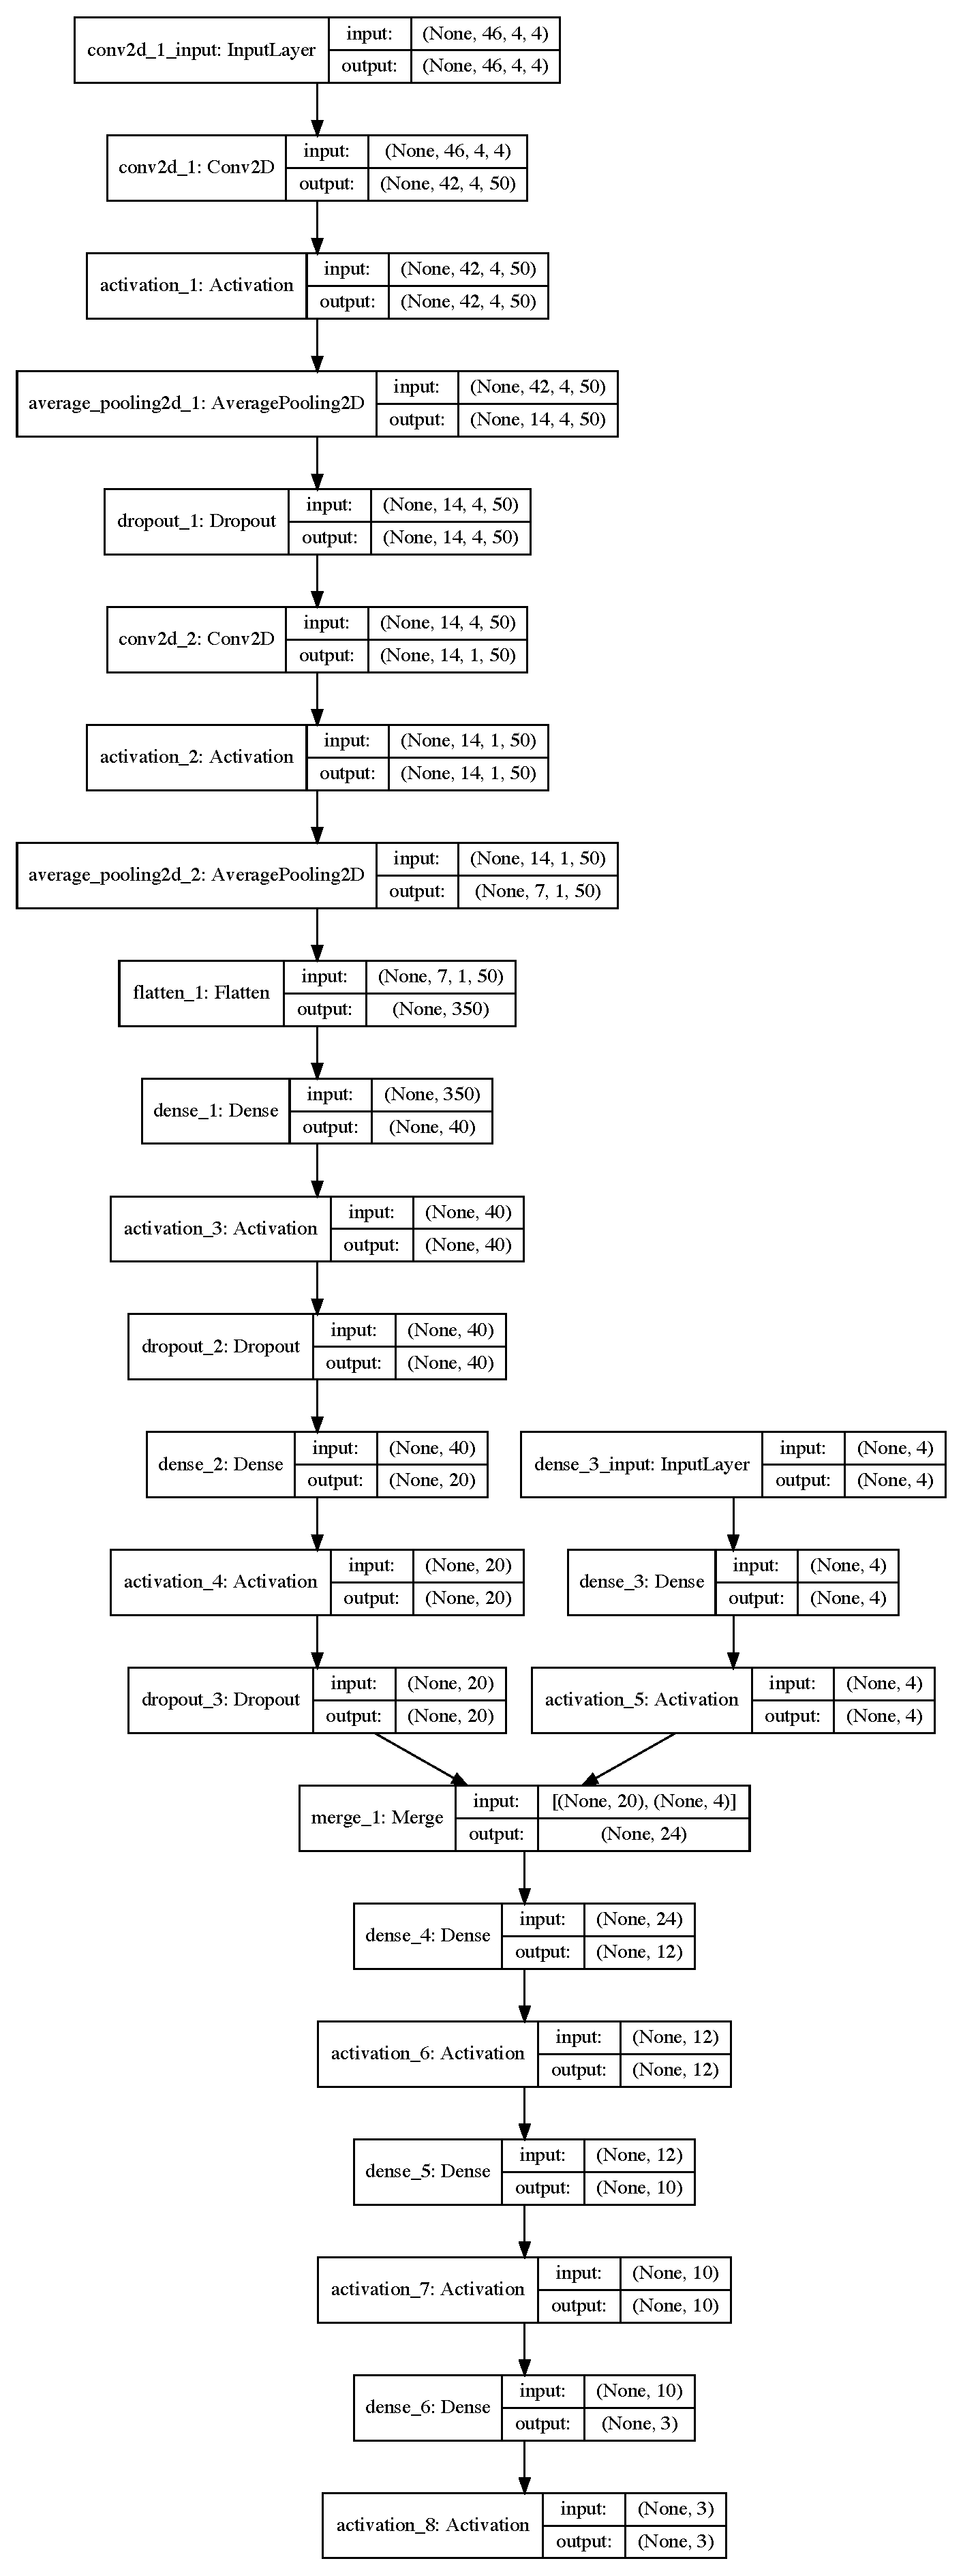
\includegraphics[width=0.6\textwidth]{Figures/Chapter5/SNAGNNoise}
  \caption{The CNN used for classification of SN vs AGN vs Noise. Each layer is labeled with its function within the network as well as its input and output dimentions.}
  \label{fig:AGNNoiseSNModel}
\end{figure}

\subsubsection{Training the model}
The combined training sample build in \sref{sec:AGNNoiseSNSample} is passed through the network using a batch size of 5000 objects with 100 epochs, or individual runs of the backpropagation algorithm. CNNs are often trained on smaller batches of data to accelerate the learning process and help to prevent overfitting. As a general rule of thumb for the choice of the number of the fitting epoch, the fitting is stopped when the model approaches convergence as an excessive number of epochs would allow the model to `learn' the test sample leading to overfitting.

My best model, as described in \sref{sec:AGNNoiseModel}, converges rapidly to the accuracy of 99.7\%. \fref{fig:AGNNoiseROC} shows the Receiver Operating Characteristic (ROC) which is the most commonly used metric of the accuracy of the classification model. The Area Under Curve (AUC) for the ROC has used an indicator that for each individual object's the probability of being a true positive vs a true negative. For this model, I have measured it to be 99.97\%.

\begin{figure}
  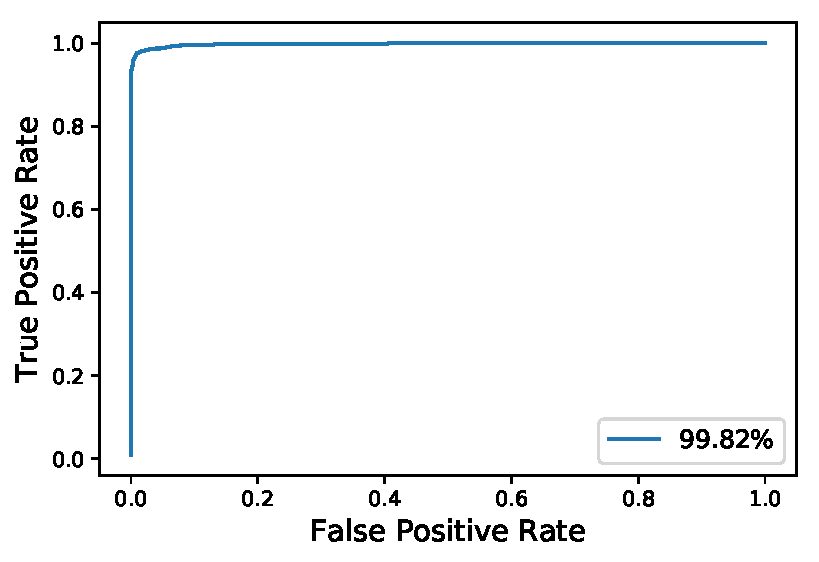
\includegraphics[width=\textwidth]{Figures/Chapter5/SNAGNNoiseROC.pdf}
  \caption{ROC curve and the AUC showing the accuracy, reflecting the high quality of the SN vs AGN vs Noise ML model introduce in this section.}
  \label{fig:AGNNoiseROC}
\end{figure}

\subsubsection{Selecting SNe}
After the numerous preparation steps, we can now obtain classifications for each real, unlabelled DES transient. 19,500 objects were sanitised and reshaped using the same method as the training sample before being passed through the classification network. Amongst this sample, 6000 objects received a classification of `most-likely' being a SN, e.g their probability was highest for this label.

To test the classification model and determine a probability threshold that would ensure a high purity of the sample, I use the samples of spectroscopically classified SNIa, CCSN, SLSNe and AGN as a ground-truth sample. Regardless of their subclass, all confirmed SN in the sample were correctly classified using our CNN and all AGN were also correctly accounted for. Furthermore, each confirmed SN has been identified with a very high degree of confidence exceeding 99\% in the worst cases with an average exceeding 99.99\% for the majority of transients. This result confirms that the high degree of accuracy could not be attributed to overfitting or errors in the analysis but was, in fact, the true representation of the quality and ability for the CNNs to differentiate these classes of transients. The high level of accuracy suggests that a similar project performed on data with lower quality or more incomplete light curves could still result in a positive result paving way for similar methods to be applied in the future astronomical surveys including LSST.

Using the classification probability values measured for the confirmed objects, I set a conservative threshold of 98\% to select objects which are to enter the next stage of my analysis. This retained 5273 objects which are an approximate match to the numbers of SN discoveries expected in DES \citep{Bernstein2012}.

\subsection{Classifying SNe}
Upon the classification of 5273 transients found in the first four years of operation of DES, the next step of the analysis is to attempt to divide these objects into their respective subclasses using only their light curve data. This task is perhaps one of the greatest challenges facing SN surveys to date, with no project ever accomplishing this with a high degree of confidence without the use of reshifting as a modelling prior.

The classification of SN in the absence of the distance prior requires us to focus purely on the morphology of the light curve including its colour and temporal evolution and apparent luminosity as the only available sources of information. These differences may be very subtle for a number of SN classes, most predominantly SN\,Ia and SN\,Ibc, and we, therefore, do not expect to be able to produce a classification model matching the accuracy of that used to identify SN candidates in DES.

\subsubsection{Data preparation and network selection} \label{sec:SNClassificationNetwork}
The training sample used in the classification of SNe is similar to that used in the previous section, albeit consisting of SN light curve only. In order to provide a fair representation for each subclass of objects, I use an equal sample of SN\,Ia, CCSN and SLSN in each case 45,000 objects from the training set. In the case of CCSNe, I use an even contribution from both the sample of SN\,II and SN\,Ibc. The data is also sanitised and reshaped using the tools as used in \sref{sec:AGNNoiseSNSample}

To build the SN classification model, I use the approach developed in \sref{sec:AGNNoiseModel} as the benchmark, modifying that network to suit this more complex problem. Perhaps the most important change was the introduction of the absolute magnitude as one of the input parameters. In the selection of SNe, performed in \sref{sec:AGNNoiseModel}, this was not necessary as the light curve evolution, normalised to one for each object, provides sufficient information to distinguish between these very distinct classes of objects. In the case of SNe, the difference is very subtle relative to the previous model with the luminosity as a function of the colour likely being one of the strongest indicators for each subclass. The absolute luminosity is measured as the maximum flux in each band across all seasons of data. This provides only four additional data points and is, therefore, introduced late into the network in order to provide more weight in determining the final classification (\fref{fig:SNClassificationNetwork}).

\begin{figure}
  \centering
  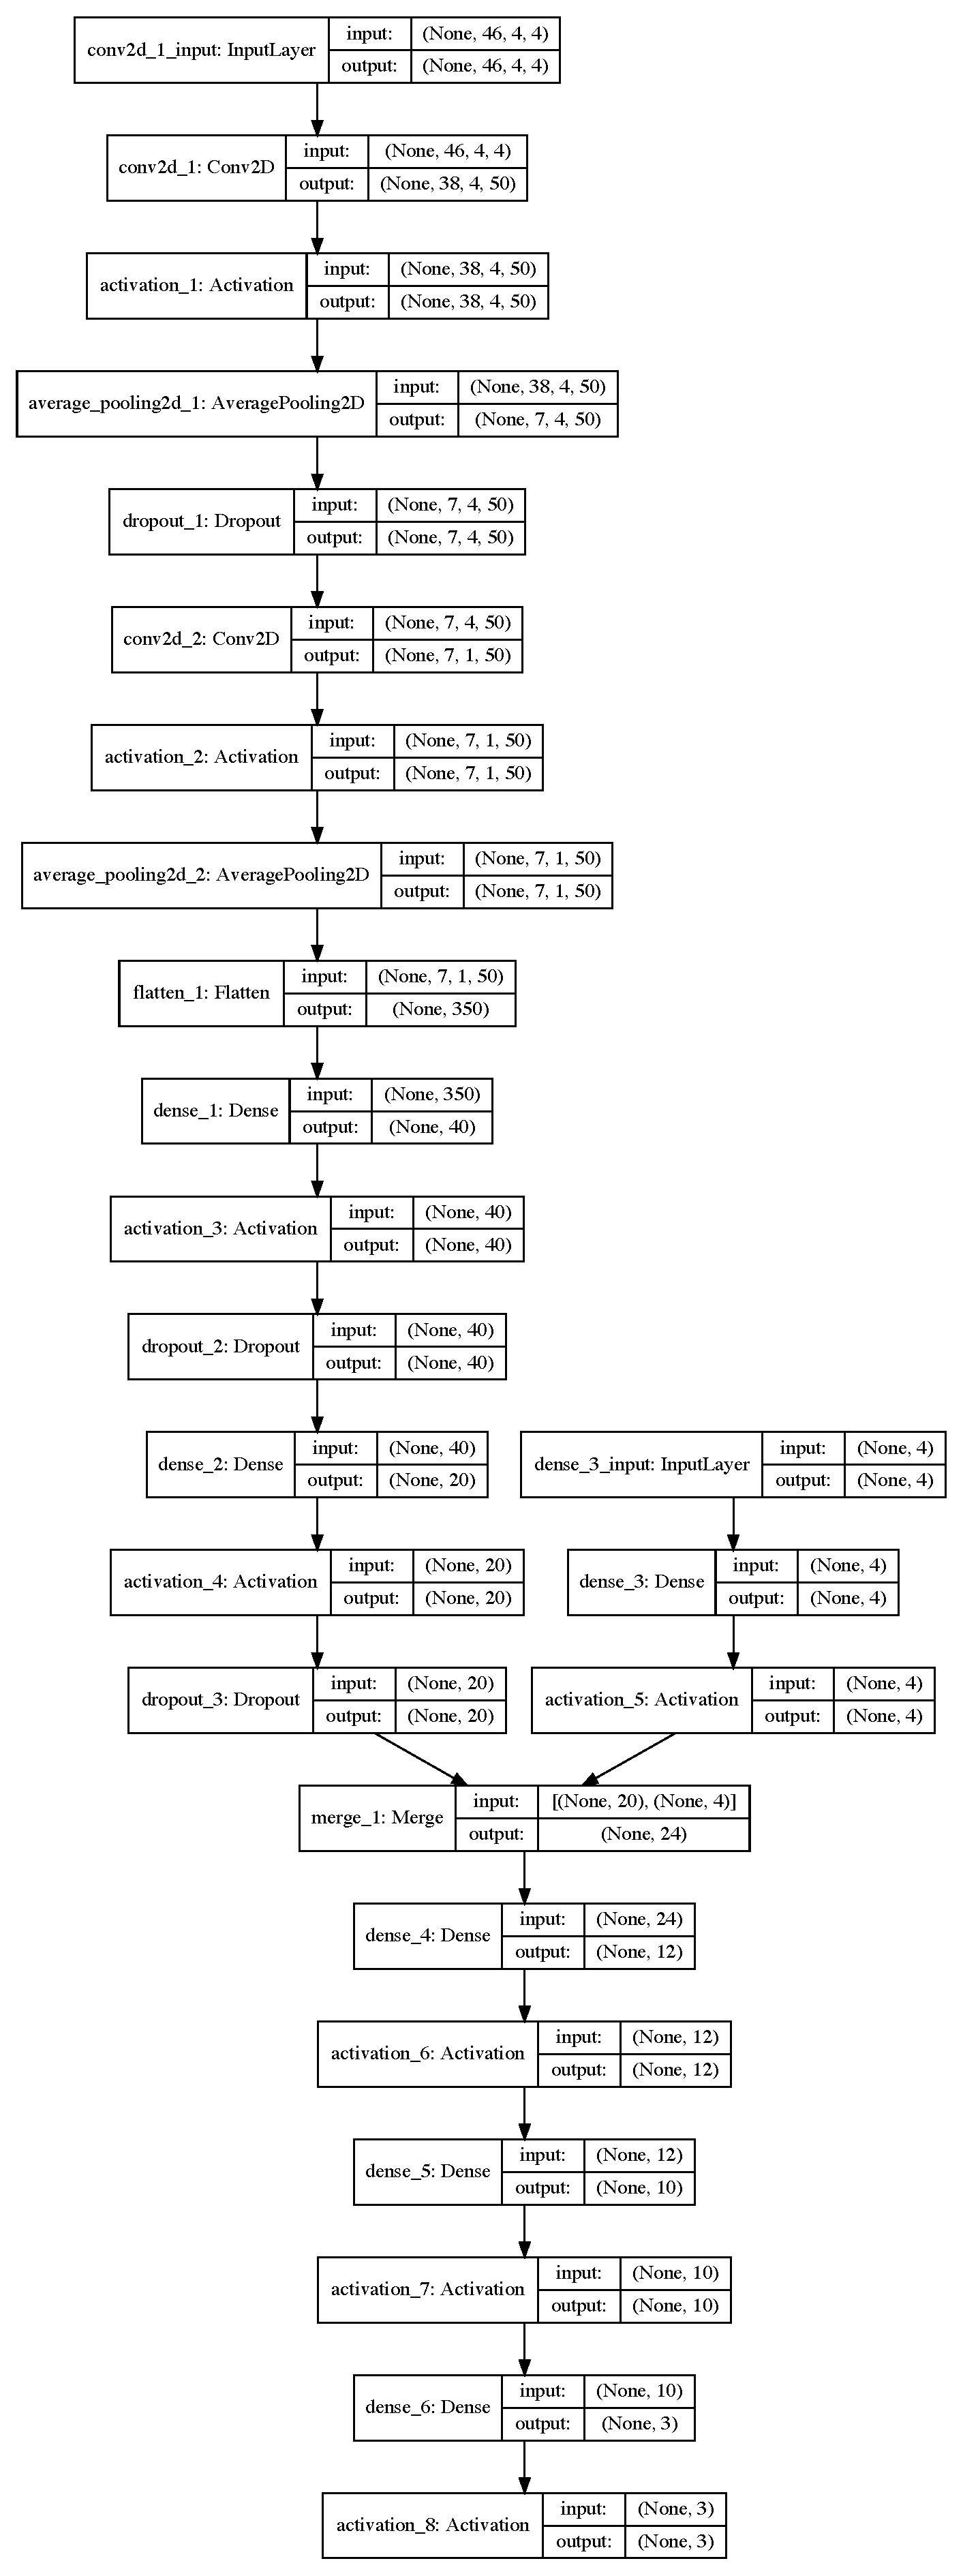
\includegraphics[width=0.6\textwidth]{Figures/Chapter5/SN}
  \caption{The CNN used to subclassify DES SNe amongst their spectral subtypes. This network relies on `Tanh' activation funtions and makes use of the information about the apparent luminosity of the SN, differing from that used in \sref{sec:AGNNoiseModel}}
  \label{fig:SNClassificationNetwork}
\end{figure}

Another important change in this iteration of the CNN was an increase in the number of convolutional filters responsible for measuring the colour of the SN. Through a number of iterations of the model, I found that an increase from 30 to 50 unique filters improves the classification rate by $\sim$3\% without overfitting the model.

Finally, one of the biggest improvements in the model came from modifying the activation function to follow the Tanh distribution over ReLU, introducing an improvement of $\sim$5\%. Interestingly, the same behaviour was not previously observed in the SN identification network, where the use of Tanh or Sigmoidal activation functions hinders the classification rate. One possible explanation of this comes from the fact that the differences between the objects in the training samples in the SN identification sample are so large that they require a more flexible and forgiving activation function such as ReLU, while the similarity of the SN subclasses requires a very sensitive, high gradient function to be used. The benefit of the Tanh over a Sigmoid is the scaling between the negative and positive unity as opposed to zero and one, which allows for objects with small negative values.

\subsubsection{Training the model} \label{sec:SNClassification}
Using the training sample and the CNN developed in \sref{sec:SNClassificationModel}, I built a SN classification model that, with an accuracy of 90\%, is one of the most successful SN classifiers to date, despite its independence from any distance priors. At the stage of classifying a purified sample of SNe, our result can be directly compared with \citet{Lochner2016}. Our AUC measured at 97.9\% for SN\,Ia marginally exceeds that of the best result found in \citet{Lochner2016}. However, this does not tell the full story as the best model found in their work sufferers largely from overfitting and the more correct value, found using a larger (albeit non-representative of all subclasses) sample is closer to $\sim$85\%. The accuracy of our classifier is again a testament to the power of CNNs, demonstrating that a similar model could be used in future surveys such as LSST.

\begin{figure}
  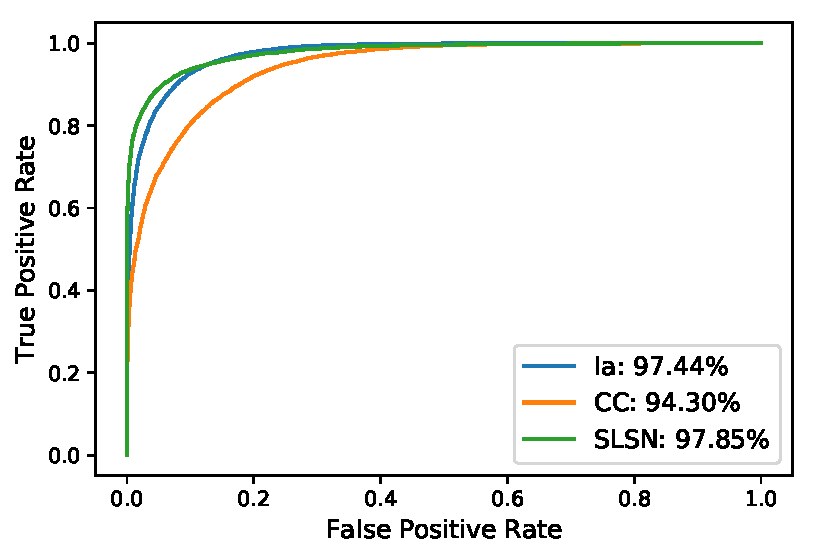
\includegraphics[width=\textwidth]{Figures/Chapter5/SNROC.pdf}
  \caption{The ROC and AUC measured for the SN photometric classification model shown separately for each class of SN present in our training sample.}
  \label{sec:SNClassificationROC}
\end{figure}

\subsection{SLSNe in DES}
Before the SN classification model can be applied to the sample of DES SN candidates, identified in \sref{sec:SNClassification}, it must first be tested against the ground-truth sample of spectroscopically confirmed objects detected by DES. While the model shows that a high degree of precision, it is possible that mistakes in the creation of the artificial training sample could lead to some subclasses not being represented correctly in the classification model.

\subsubsection{Ground-truth sample} \label{sec:SNTruth}
Amongst the sample of 250 spectroscopically confirmed SN\,Ia, 243 are correctly classified in this work. This, in fact, exceeds the value expected from the raw accuracy figures, which are likely explained by the spectroscopically confirmed objects being easier to classify than some objects that may lay at the detection limit of the survey.

With this positive result, I apply the same method to SN\,Ib/c and SN\,II. Here the results begin to shed a light on a major issue uncovered in this section. While a majority of the SN\,Ib/c have been correctly identified, a number of SN\,II have been misidentified as SLSN. The visual inspection of these objects shows that they are exclusively SN\,IIP, with particularly slow descent times. This is a subclass of objects which was not represented in the training sample due to the lack of sufficient data. At the current time, using the data available in the literature it is not possible to expand our training set with examples of SN\,IIP. However, in \cref{Chapter6} I investigate other approaches, centred around the concept of Unsupervised ML to separate these two groups of transients and provide a pure sample of SLSN.

As a final check, I test the sample of DES SLSNe and find that 12 of the 18 objects are fully recovered by the model. While at the first glance, this appears to be in contradiction with the predicted accuracy of the classifier, two of these objects are known to be only tentatively classified as SLSN (DES15C3hav, DES14C1rhg). Three objects are known not to be a good match to the magnetar model under any assumptions tested in \sref{sec:MagnetarModel} (DES13S2cmm, DES14S2qri). It is harder to postulate why DES16C3ggu and DES15X1noe are not part of the sample.

\begin{table}
  \caption{Percentage probability of the spectroscopically confirmed DES SLSNe as found in the ML photometric classification presented in this chapter.}
  \label{tab:SLSNTruth}
  \centering
  \begin{tabular}{l|r|r|r}
    SN Name & SN\,Ia & CCSN & SLSN \\
    \hline
    DES13S2cmm & 0.04\,\% & 89.18\,\% & 10.77\,\% \\
    DES15X3hm  & 5.65\,\% & 7.40\,\% & 86.95\,\% \\
    DES14X3taz & 1.71\,\% & 2.25\,\% & 96.04\,\% \\
    DES15S2nr  & 0.01\,\% & 0.54\,\% & 99.46\,\% \\
    DES14C1fi  & 0.00\,\% & 0.11\,\% & 99.89\,\% \\
    DES14X2byo & 0.01\,\% & 0.10\,\% & 99.89\,\% \\
    DES15C3hav & 46.10\,\% & 10.38\,\% & 43.52\,\% \\
    DES14C1rhg & 0.87\,\% & 96.90\,\% & 2.23\,\% \\
    DES14S2qri & 2.92\,\% & 90.66\,\% & 6.43\,\% \\
    DES14E2slp & 0.28\,\% & 1.85\,\% & 97.87\,\% \\
    DES15E2mlf & 0.00\,\% & 0.23\,\% & 99.77\,\% \\
    DES15X1noe & 3.63\,\% & 52.81\,\% & 43.56\,\% \\
    DES15S1nog & 19.93\,\% & 14.05\,\% & 66.02\,\% \\
    DES16C3cv  & 0.00\,\% & 0.04\,\% & 99.96\,\% \\
    DES16C2nm  & 0.00\,\% & 0.05\,\% & 99.95\,\% \\
    DES16C2aix & 0.05\,\% & 46.19\,\% & 53.76\,\% \\
    DES16C3dmp & 9.60\,\% & 3.51\,\% & 86.89\,\% \\
    DES16C3ggu & 85.20\,\% & 11.52\,\% & 3.28\,\%
  \end{tabular}
\end{table}

\subsubsection{SN classification}
I applied the final classification model to the 5273 objects real DES objects, previously identified as SN candidates. At the 50\% accuracy threshold, 3192 objects were identified as SN\,Ia which matches the expected values found in \citep{Bernstein2012}, 1389 objects were identified as CCSN which again does not exceed our expectations. The remaining 509 objects were identified as SLSN.

This exceeds the numbers expected from the rate of SLSN and is known to be contaminated with long duration SN\,II. However, as the classification model was shown in \sref{sec:SNTruth} to be able to identify a number of known SLSN with a high degree of accuracy (\tref{SLSNTruth}), we have a strong degree of belief that there are in fact numerous SLSN hidden in this contaminated sample that may be recoverable using further analysis, presented in \cref{Chapter6}

\section{Summary}
In this chapter, I described the approach used in building a training sample of transients resembling the sample of real transients observed by the DES. I used the SNANA generated sample of SN\,Ia. The CoCo and SLAP packages, developed in \cref{Chapter3}, were used to create samples of CCSN and SLSNe respectively. Furthermore, I use a sample of AGNs generated for a similar study in \citet{Hoenig2014} and a basic model of spurious noise detections to generate a DES-like sample of real transients and their contaminants. I use the approach similar to that found in SNANA to apply the survey noise to the modelled light curves before augmenting them to a uniform cadence using GPR, previously discussed in \sref{sec:Augmentation}.

This training sample was used to develop a classification pipeline for photometrically identifying a sample of real SN candidates in DES. This was performed in conjunction with the state of the art CNN algorithm. A similar approach was subsequently used to create a SN photometric classification tool. Our testing suggests that it is one of the most powerful tools of its kind currently available. I applied it to the DES dataset identifying 3192 SN\,Ia, 1389 potential CCSN and a sample of 500 SLSN, although we understand that this sample is heavily contaminated by SN\,IIP which were not included in the original training sample.
